\documentclass[letterpaper]{article}

\usepackage{geometry}
\newgeometry{vmargin={25mm}, hmargin={30mm,30mm}}

\setcounter{secnumdepth}{0}

\usepackage{noto}
\usepackage{CJKutf8}
\usepackage[T1]{fontenc}

\usepackage{amsmath}
\usepackage{listings}
\usepackage{xcolor}
\usepackage{multirow}
\usepackage{float,graphicx}
\usepackage{subcaption}
\usepackage[breaklinks=true]{hyperref}
\usepackage{etoolbox}
\appto\UrlBreaks{\do\-}

\usepackage{mdframed}
\newenvironment{modeloutput}[1]{%
	\begin{mdframed}[backgroundcolor=gray!8, linecolor=gray!60, linewidth=0.8pt,
		innerleftmargin=8pt, innerrightmargin=8pt, innertopmargin=6pt, innerbottommargin=6pt]%
		\small\ttfamily\raggedright
	}{%
	\end{mdframed}%
}

\lstset{
	basicstyle=\small\ttfamily,
	tabsize=4,
	frame=single,
	breaklines,
	postbreak=\mbox{\textcolor{red}{$\hookrightarrow$}\space},
	showstringspaces=false,
}

\newcommand{\repofile}[2]{\href{https://github.com/echung32/ece405-assignment3-alignment/blob/main/#1}{#2}}
\graphicspath{{report/figures/}{figures/}}

\begin{document}
	\title{Assignment 3: Alignment}
	
	\author{Ethan Chung\\
		{\tt\small University of Hawaii}\\
		{\tt\small ECE 405: Intro to Large-Scale AI Systems}\\
		{\tt\small [redacted]@hawaii.edu}}
	
	\maketitle
	
	\tableofcontents
	
	\newpage
	
	\section{Measuring Zero-Shot MATH Performance}
	
	\subsection{Problem (math\_baseline): 4 points}
	
	\begin{itemize}
		\item[(a)] Write a script to evaluate Qwen 2.5 Math 1.5B zero-shot performance on MATH.
		
		\textit{Implemented in \repofile{cs336_alignment/math_baseline.py}{cs336\_alignment/math\_baseline.py}.}
		
		\item[(b)] Run your evaluation script on Qwen 2.5 Math 1.5B. How many model generations fall into each of the following categories: (1) correct with both format and answer reward 1, (2) format reward 1 and answer reward 0, (3) format reward 0 and answer reward 0? Observing at least 10 cases where format reward is 0, do you think the issue is with the base model’s output, or the parser? Why? What about in (at least 10) cases where format reward is 1 but answer reward is 0?
		
		Running the baseline on the validation split (single-GPU vLLM) produced 1{,}250 generations: 27 \texttt{correct\_with\_format}, 173 \texttt{formatted\_but\_incorrect}, and 1{,}050 \texttt{unformatted}. Formatting errors clearly dominate over near-miss mathematical mistakes. A typical correct case follows the expected structure exactly, e.g.\ a digit puzzle where the model outputs \texttt{1</think> <answer>3</answer>} and receives reward $(1.0, 1.0, 1.0)$.
		
		Inspecting unformatted outputs suggests the issue lies primarily with the base model rather than the parser. Many responses fail to emit valid answer tags despite otherwise reasonable reasoning. For example, in a problem asking for $|{-324} + 243i|$, the model produces \texttt{We start with <answer=\_\$ </answer>}, which yields reward $(0.0, 0.0, 0.0)$ because the tag is malformed and no valid answer span is detected. Quantitatively, among the 1{,}050 unformatted cases, 330 contain both tags but often misplaced, 152 include only an opening \texttt{<answer>} tag, 240 contain code blocks, and 58 prepend strings such as \texttt{Assistant: <answer>}. These patterns indicate generation errors—failure to follow the required format—rather than parser issues.
		
		For \texttt{formatted\_but\_incorrect} cases, the failures are mostly due to reasoning or answer expression. The model typically produces a valid tagged answer, but it is numerically incorrect, incomplete, or not in the expected canonical form. For instance, in a cube-rolling path problem, the model outputs \texttt{7/6pi</think> <answer>7/6</answer>} with reward $(0.0, 1.0, 0.0)$: the format is correct, but the final answer omits the factor of $\pi$. Similar cases include returning intermediate values or placing extraneous text inside the answer tags. These errors point to issues with mathematical correctness and normalization rather than parsing.
		
		\item[(c)] How well does the Qwen 2.5 Math 1.5B zero-shot baseline perform on MATH?
		
		On the validation split, the zero-shot baseline reached mean answer reward 0.0216, mean total reward 0.0216, and mean format reward 0.16. In other words, only 2.16\% of validation problems were solved correctly under the provided reward function, and the much larger gap between format success (16\%) and final correctness shows that both prompt-following and mathematical reasoning are weak in this zero-shot setting.
		
	\end{itemize}
	
	\section{Supervised Finetuning for MATH}
	
	\subsection{Problem (tokenize\_prompt\_and\_output): Prompt and output tokenization}
	
	\begin{itemize}
		\item[(a)] Implement a method \texttt{tokenize\_prompt\_and\_output} that tokenizes the question and output separately, concatenates them together, and constructs a response mask.
		
		\textit{Implemented in \repofile{cs336_alignment/section4/tokenize_prompt_and_output.py}{cs336\_alignment/section4/tokenize\_prompt\_and\_output.py}.}
		
	\end{itemize}
	
	\subsection{Problem (compute\_entropy): Per-token entropy}
	
	\begin{itemize}
		\item[(a)] Implement a method \texttt{compute\_entropy} that computes the per-token entropy of next-token predictions.
		
		\textit{Implemented in \repofile{cs336_alignment/section4/compute_entropy.py}{cs336\_alignment/section4/compute\_entropy.py}.}
		
	\end{itemize}
	
	\subsection{Problem (get\_response\_log\_probs): Response log-probs (and entropy)}
	
	\begin{itemize}
		\item[(a)] Implement a method \texttt{get\_response\_log\_probs} that gets per-token conditional log-probabilities from a causal language model, and optionally the entropy of the model’s next-token distribution.
		
		\textit{Implemented in \repofile{cs336_alignment/section4/get_response_log_probs.py}{cs336\_alignment/section4/get\_response\_log\_probs.py}.}
		
	\end{itemize}
	
	\subsection{Problem (masked\_normalize): Masked normalize}
	
	\begin{itemize}
		\item[(a)] Implement a method \texttt{masked\_normalize} that sums over tensor elements and normalizes by a constant while respecting a boolean mask.
		
		\textit{Implemented in \repofile{cs336_alignment/section4/masked_normalize.py}{cs336\_alignment/section4/masked\_normalize.py}.}
		
	\end{itemize}
	
	\subsection{Problem (sft\_microbatch\_train\_step): Microbatch train step}
	
	\begin{itemize}
		\item[(a)] Implement a single micro-batch update for SFT, including cross-entropy loss, summing with a mask, and gradient scaling.
		
		\textit{Implemented in \repofile{cs336_alignment/section4/sft_microbatch_train_step.py}{cs336\_alignment/section4/sft\_microbatch\_train\_step.py}.}
		
	\end{itemize}
	
	\subsection{Problem (log\_generations): Logging generations}
	
	\begin{itemize}
		\item[(a)] Implement a function \texttt{log\_generations} that can be used to log generations from your model.
		
		\textit{Implemented in \repofile{cs336_alignment/section4/log_generations.py}{cs336\_alignment/section4/log\_generations.py}.}
		
	\end{itemize}
	
	\subsection{Problem (sft\_experiment): Run SFT on the MATH dataset}
	
	\begin{itemize}
		\item[(a)] Run SFT on the reasoning SFT examples, varying the number of unique examples for SFT in the range \{128, 256, 512, 1024\}, along with using the full dataset. Tune the learning rate and batch size to achieve at least 15\% validation accuracy when using the full dataset.
		
		As shown in Figure~\ref{sec4_sft_datasize}, the fixed-\texttt{2e-5} dataset-size sweep indicates that the full 10{,}000-example dataset performs best, reaching a peak validation accuracy of 0.4920. A subsequent learning-rate sweep on the full dataset (Figure~\ref{sec4_sft_lrtune}) further improves performance to 0.5064 at a learning rate of \texttt{2e-5}, with the best checkpoint at step 750.
		
		\begin{figure}[H]
			\centering
			\begin{subfigure}[t]{0.49\textwidth}
				\centering
				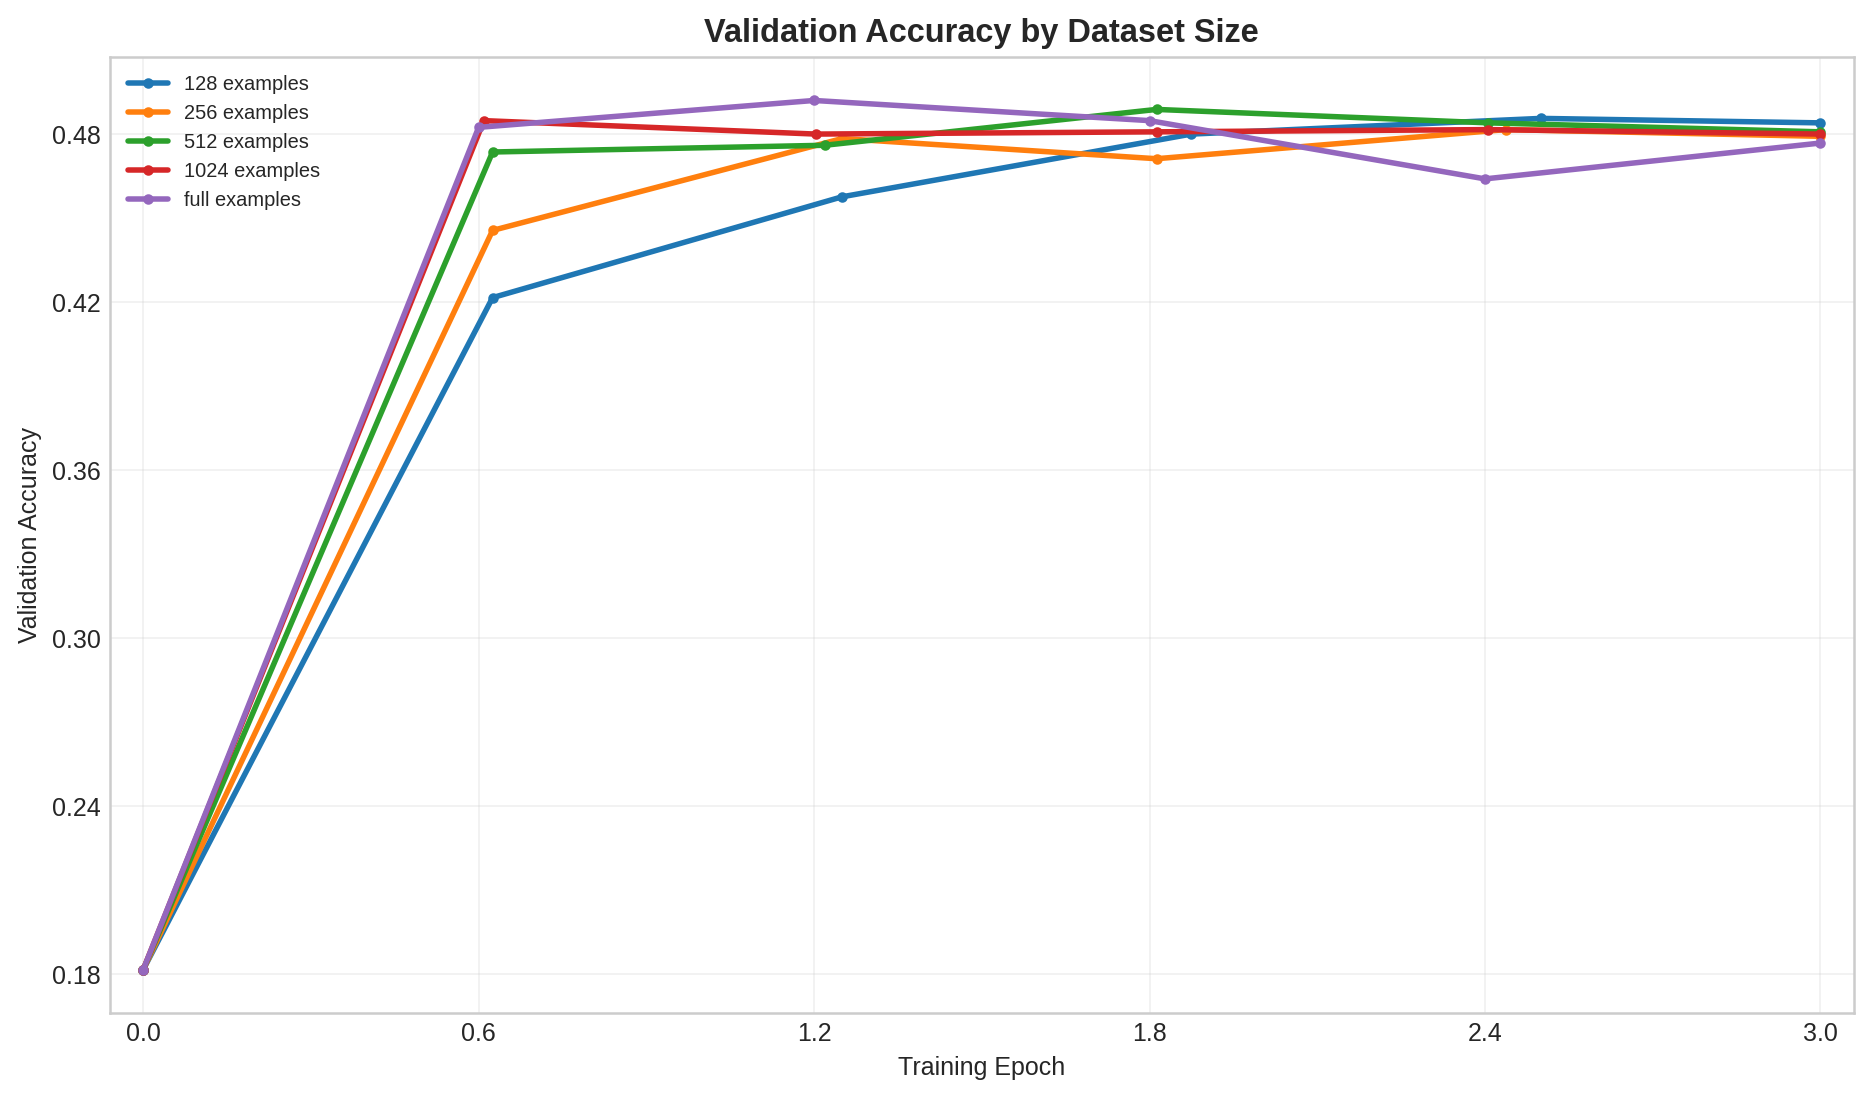
\includegraphics[width=\textwidth]{section4_dataset_size.png}
				\caption{Validation accuracy by SFT dataset size.}
				\label{sec4_sft_datasize}
			\end{subfigure}
			\hfill
			\begin{subfigure}[t]{0.49\textwidth}
				\centering
				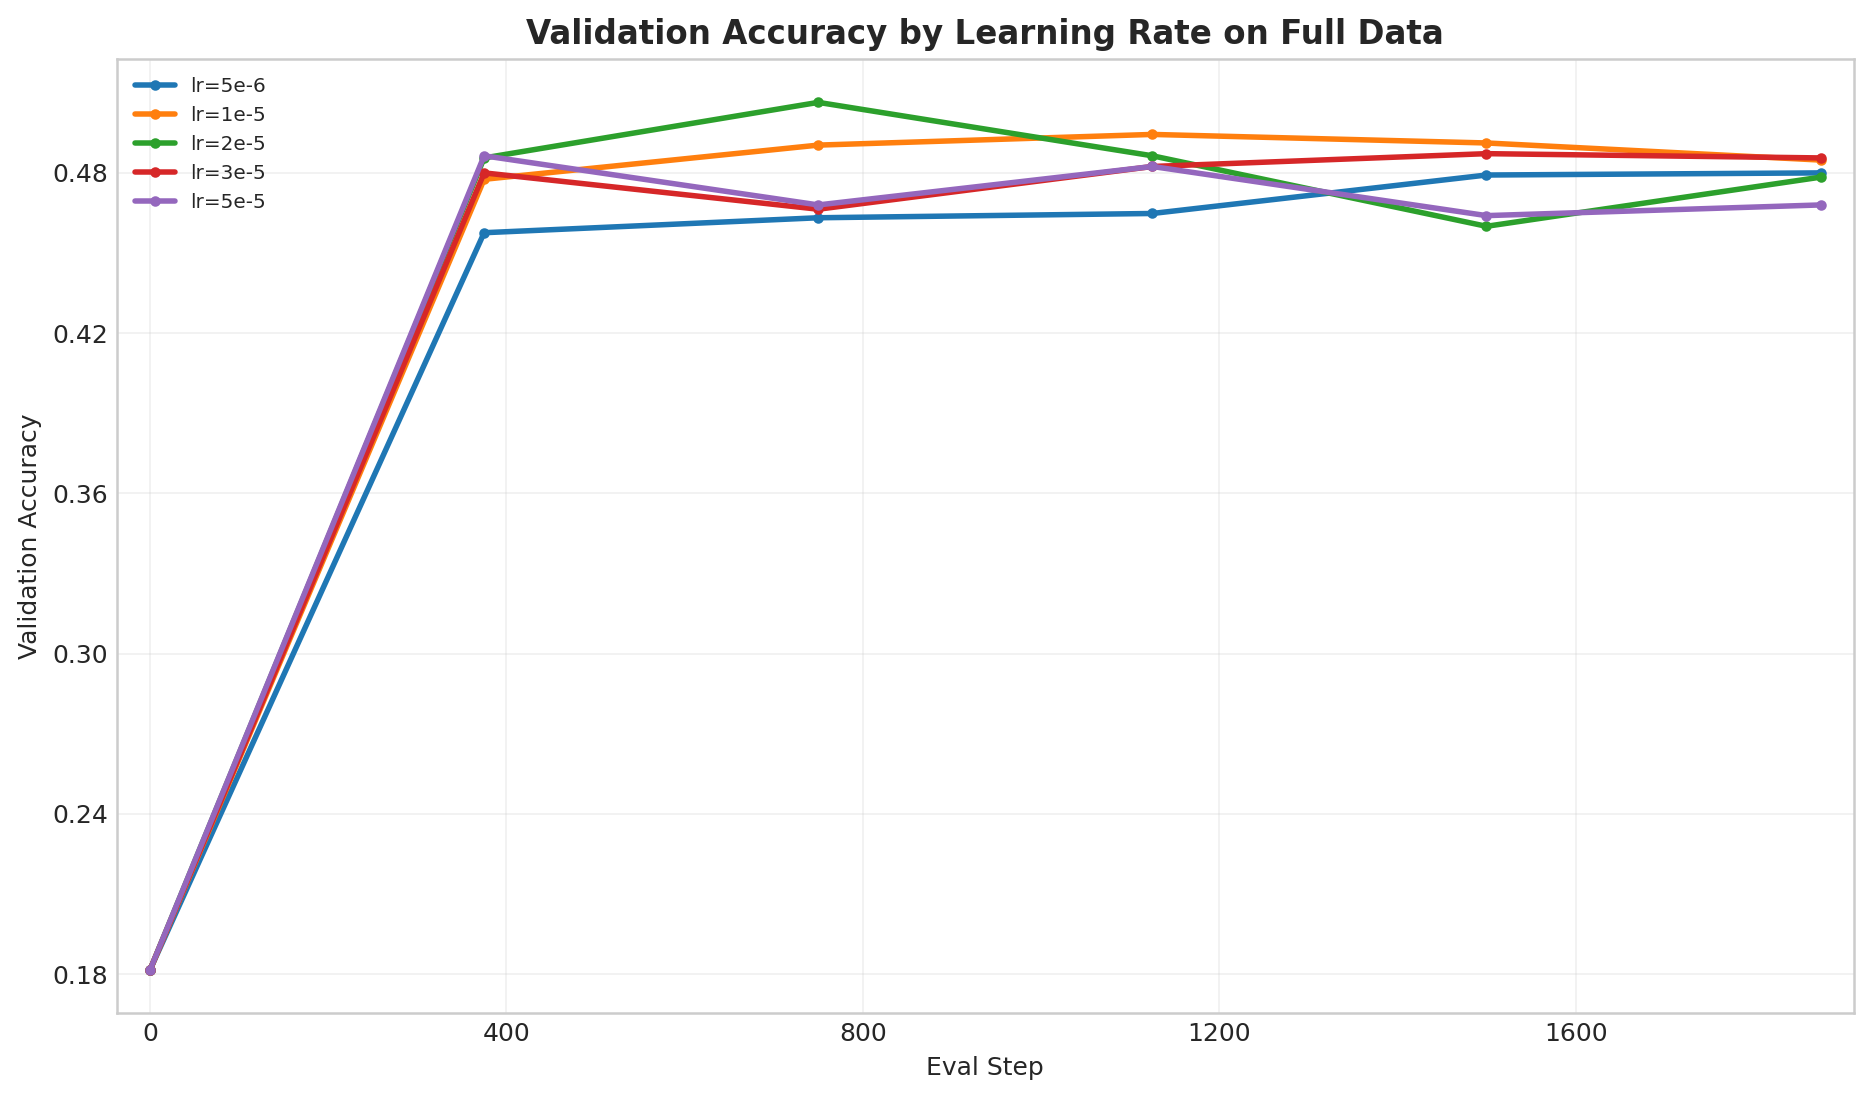
\includegraphics[width=\textwidth]{section4_learning_rate.png}
				\caption{Validation accuracy by learning rate on the full SFT dataset.}
				\label{sec4_sft_lrtune}
			\end{subfigure}
			\caption{Section 4 SFT scaling and learning-rate comparisons.}
		\end{figure}
		
		\item[(b)] Filter the reasoning SFT examples to only include examples that produce the correct answer. Run SFT on the (full) filtered dataset and report the size of the filtered dataset and the validation accuracy you achieve. Compare your findings to the previous SFT experiment.
		
		Filtering removed only two examples, yielding a filtered dataset size of 9,998. In this artifact slice, filtering slightly hurt rather than helped raw SFT performance: the filtered run reached a peak validation accuracy of 0.4848 versus 0.5064 for the best unfiltered full-data run, a drop of 0.0216. This suggests that for this model size and regime, simple correctness filtering did not buy a better warm-start and may have reduced useful response diversity.
		
		\begin{figure}[H]
			\centering
			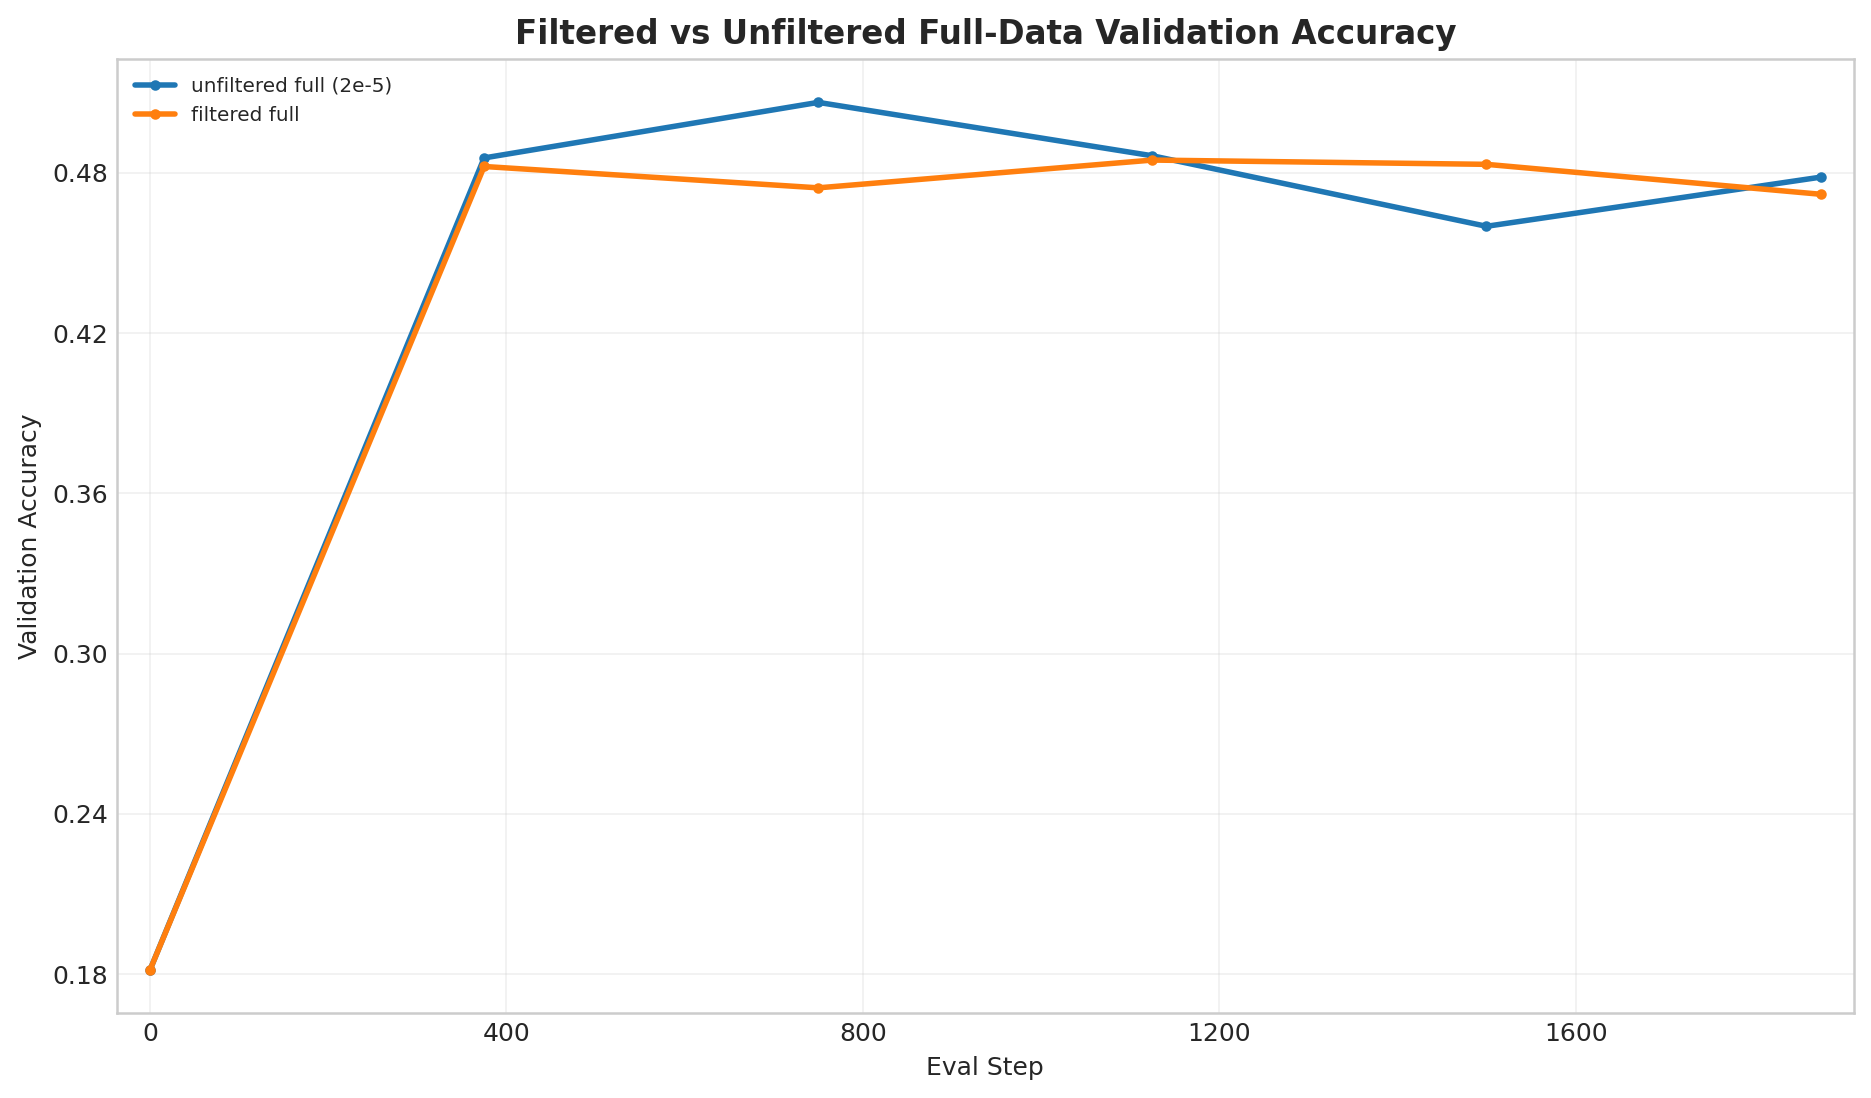
\includegraphics[width=0.8\textwidth]{section4_filtered_vs_unfiltered.png}
			\caption{Validation accuracy for filtered versus unfiltered full-data SFT.}
		\end{figure}
		
		\textit{Implementation Note}
		
		Unlike the assignment's suggested \texttt{init\_vllm} and \texttt{load\_policy\_into\_vllm\_instance}, we remove the monkeypatching code, as it no longer appears necessary in vLLM v0.19.0 (the assignment targets v0.7.2). This change may still introduce subtle differences in system behavior, so we note it here for completeness.
		
		\textit{Implemented in  \repofile{cs336_alignment/section4/sft_experiment.py}{cs336\_alignment/section4/sft\_experiment.py}.}
		
	\end{itemize}
	
	\section{Expert Iteration for MATH}
	
	\subsection{Problem (expert\_iteration\_experiment): Run expert iteration on the MATH dataset}
	
	\begin{itemize}
		\item[(a)] Run expert iteration on the MATH dataset, varying the number of rollouts and the number of SFT epochs per EI step. Log the entropy of the model’s responses over training.
		
		The sweep explored two rollout counts (4 and 8), two SFT epoch settings (1 and 2), and multiple question batch sizes. The best configuration (\texttt{group 8, db 1024, epochs 2, EI 5}) achieved 0.5117 validation accuracy at EI step 5, a modest improvement of +0.0053 over the best SFT checkpoint (0.5064).
		
		Performance across EI steps was not uniformly monotonic: stronger configurations continued improving over more iterations, while weaker ones peaked earlier and then plateaued or declined. The best run also attained the lowest entropy at its peak (0.2250), consistent with the policy becoming more confident as it concentrates on high-quality traces.
		
		\begin{figure}[H]
			\centering
			\begin{subfigure}[t]{0.49\textwidth}
				\centering
				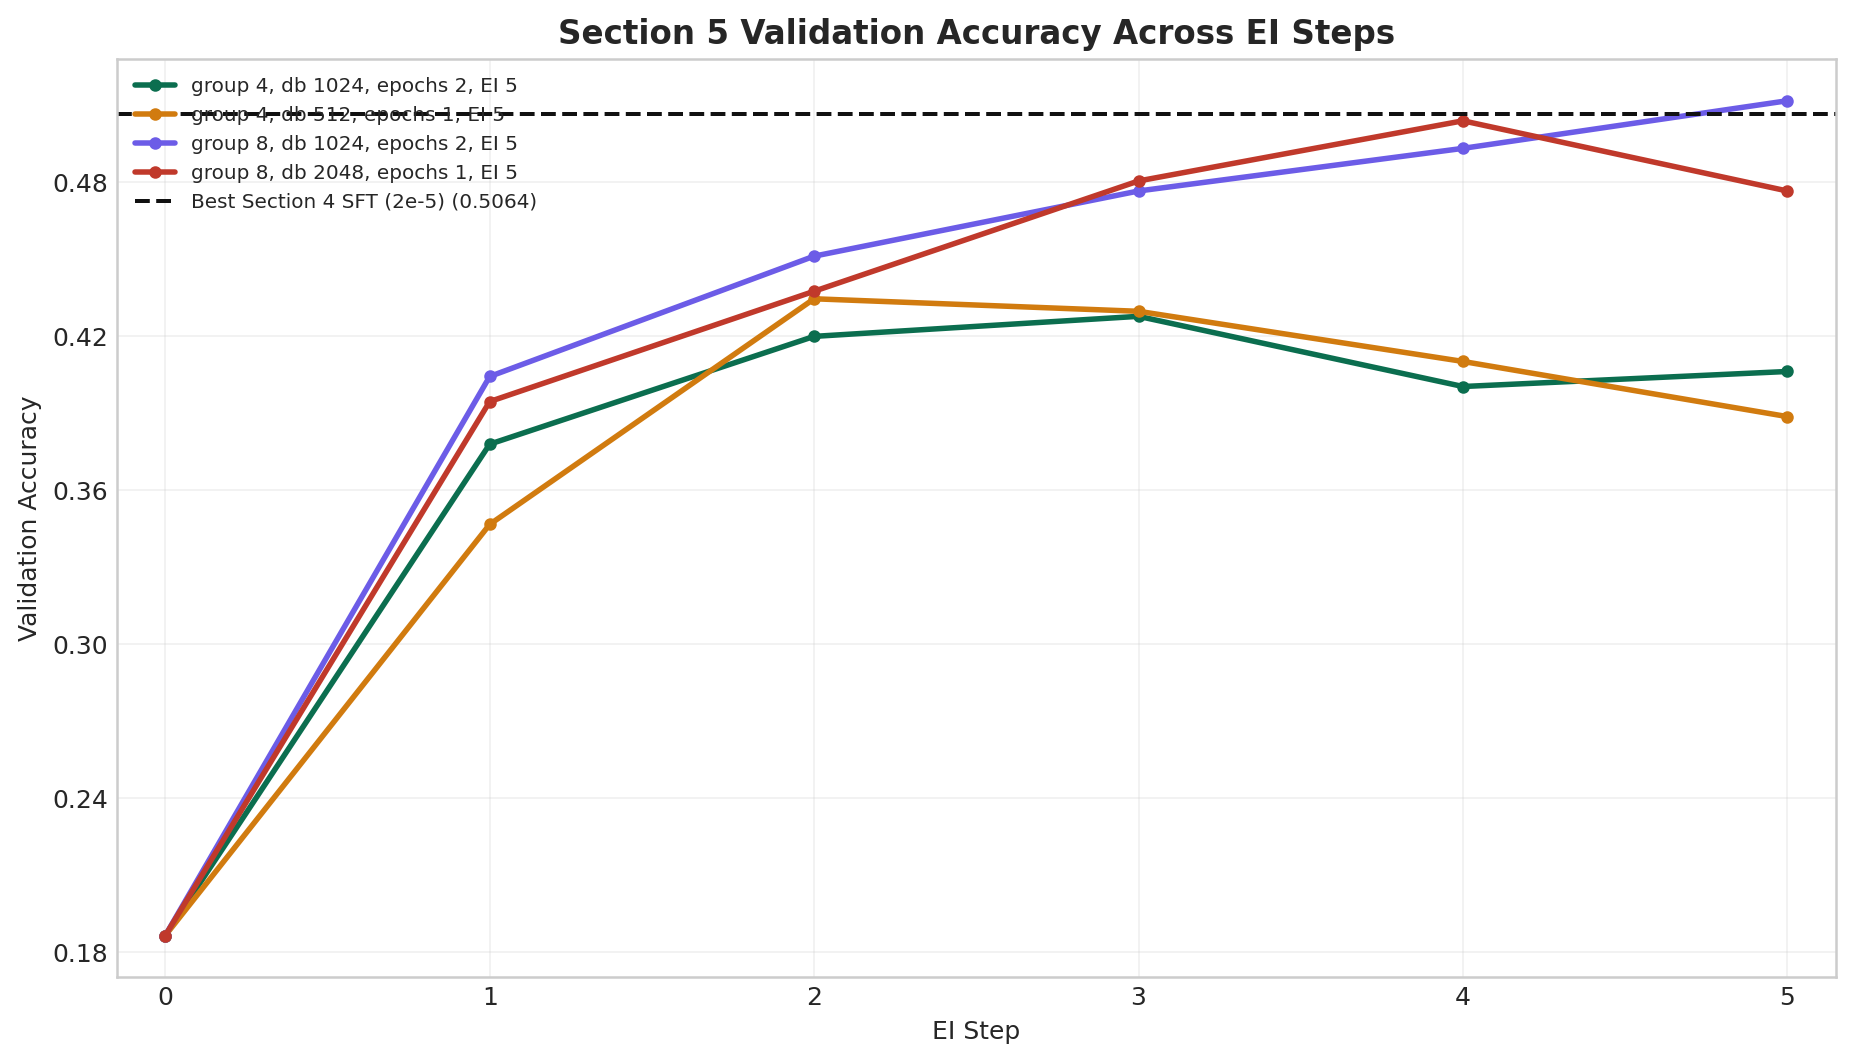
\includegraphics[width=\textwidth]{section5_validation_accuracy.png}
				\caption{Validation accuracy across EI configurations.}
			\end{subfigure}
			\hfill
			\begin{subfigure}[t]{0.49\textwidth}
				\centering
				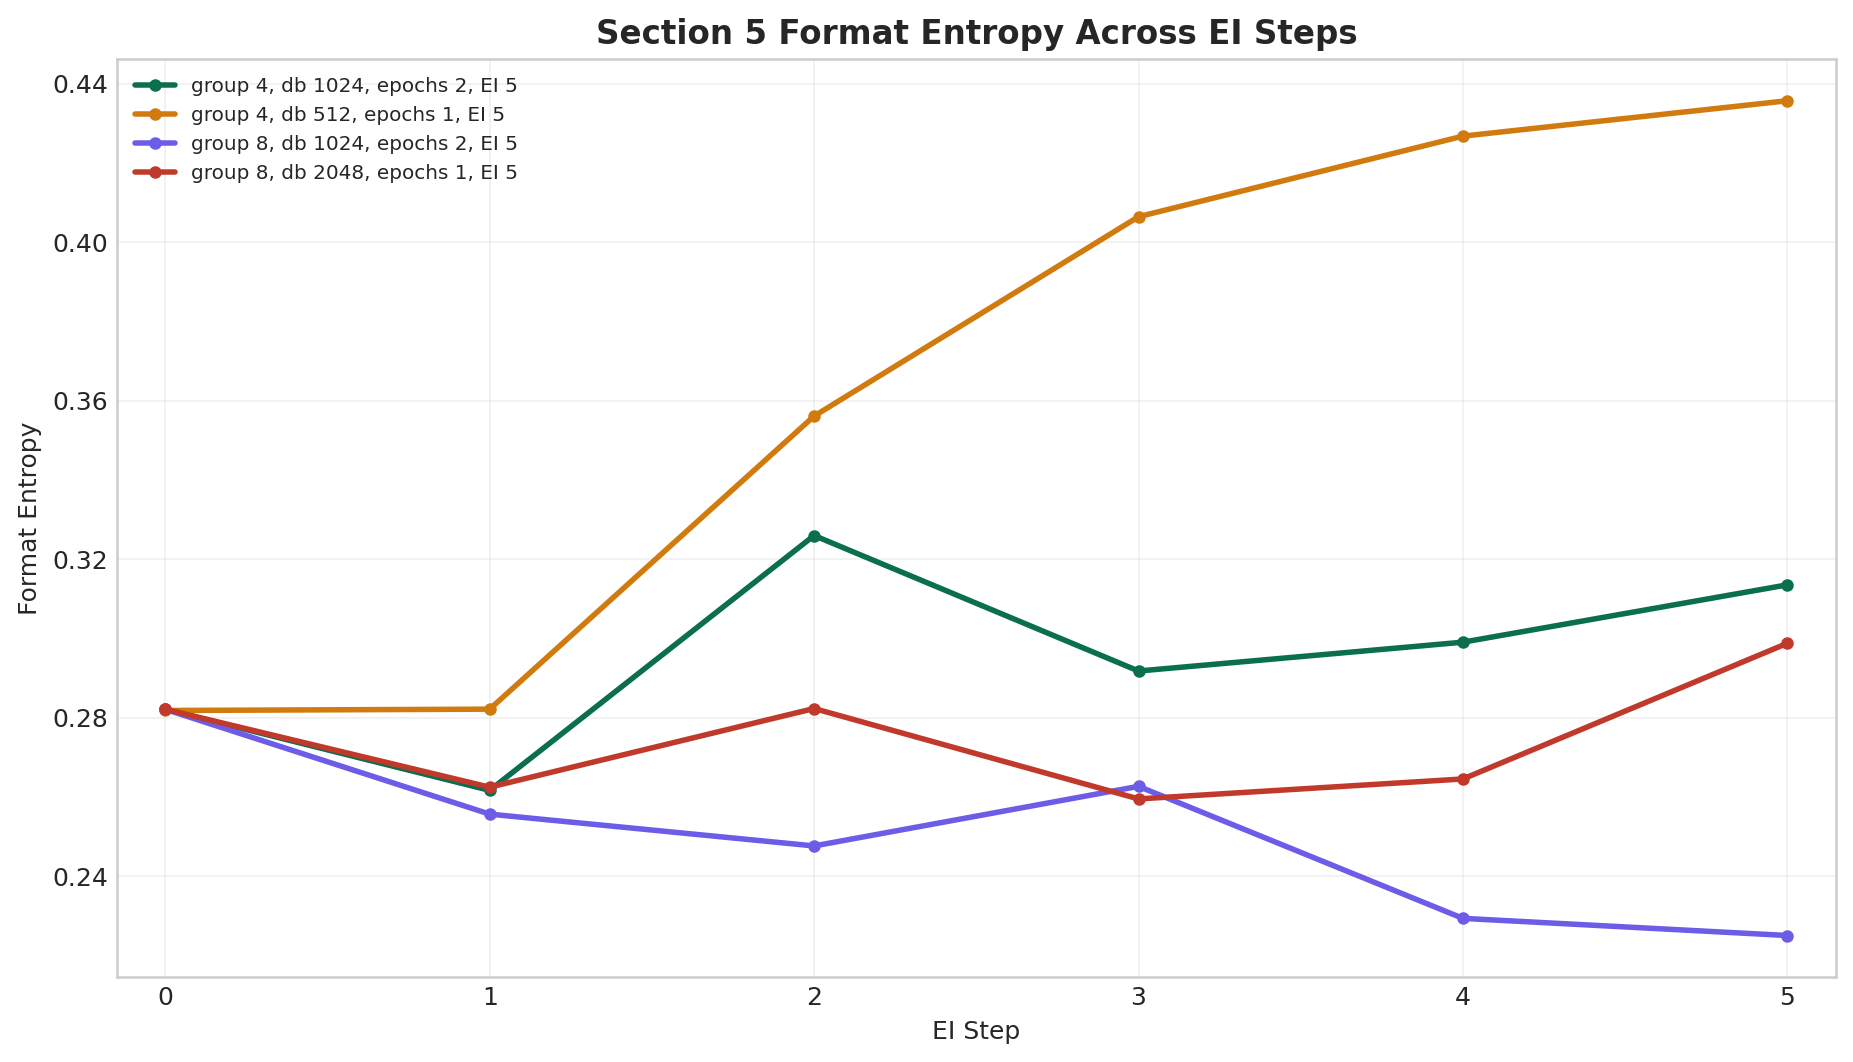
\includegraphics[width=\textwidth]{section5_entropy.png}
				\caption{Response entropy across EI configurations.}
			\end{subfigure}
			\caption{Section 5 expert-iteration validation accuracy and entropy.}
		\end{figure}
		
		\textit{Implemented in \repofile{cs336_alignment/section5/expert_iteration_experiment.py}{cs336\_alignment/section5/expert\_iteration\_experiment.py}.}
		
	\end{itemize}
	
	\section{Policy Gradient and GRPO Implementation}
	
	\subsection{Problem (compute\_group\_normalized\_rewards): Group normalization}
	
	\begin{itemize}
		\item[(a)] Implement a method \texttt{compute\_group\_normalized\_rewards} that calculates raw rewards, grouped means, and grouped normalized advantages.
		
		\textit{Implemented in \repofile{cs336_alignment/section7/compute_group_normalized_rewards.py}{cs336\_alignment/section7/compute\_group\_normalized\_rewards.py}.}
		
	\end{itemize}
	
	\subsection{Problem (compute\_naive\_policy\_gradient\_loss): Naive policy gradient}
	
	\begin{itemize}
		\item[(a)] Implement a method \texttt{compute\_naive\_policy\_gradient\_loss} that computes the token-level REINFORCE objective.
		
		\textit{Implemented in \repofile{cs336_alignment/section7/compute_naive_policy_gradient_loss.py}{cs336\_alignment/section7/compute\_naive\_policy\_gradient\_loss.py}.}
		
	\end{itemize}
	
	\subsection{Problem (compute\_grpo\_clip\_loss): GRPO-Clip loss}
	
	\begin{itemize}
		\item[(a)] Implement a method \texttt{compute\_grpo\_clip\_loss} that computes the clipped GRPO objective.
		
		\textit{Implemented in \repofile{cs336_alignment/section7/compute_grpo_clip_loss.py}{cs336\_alignment/section7/compute\_grpo\_clip\_loss.py}.}
		
	\end{itemize}
	
	\subsection{Problem (compute\_policy\_gradient\_loss): Policy-gradient wrapper}
	
	\begin{itemize}
		\item[(a)] Implement \texttt{compute\_policy\_gradient\_loss}, a convenience wrapper that dispatches between the different loss types.
		
		\textit{Implemented in \repofile{cs336_alignment/section7/compute_policy_gradient_loss.py}{cs336\_alignment/section7/compute\_policy\_gradient\_loss.py}.}
		
	\end{itemize}
	
	\subsection{Problem (masked\_mean): Masked mean}
	
	\begin{itemize}
		\item[(a)] Implement a method \texttt{masked\_mean} that averages tensor elements while respecting a mask.
		
		\textit{Implemented in \repofile{cs336_alignment/section7/masked_mean.py}{cs336\_alignment/section7/masked\_mean.py}.}
		
	\end{itemize}
	
	\subsection{Problem (grpo\_microbatch\_train\_step): Microbatch train step}
	
	\begin{itemize}
		\item[(a)] Implement a single micro-batch update for GRPO, including policy-gradient loss, masking, and gradient scaling.
		
		\textit{Implemented in \repofile{cs336_alignment/section7/grpo_microbatch_train_step.py}{cs336\_alignment/section7/grpo\_microbatch\_train\_step.py}.}
		
	\end{itemize}
	
	\subsection{Problem (grpo\_train\_loop): GRPO train loop}
	
	\begin{itemize}
		\item[(a)] Implement a complete train loop for GRPO. Begin training a policy on MATH and confirm that validation rewards improve, along with sensible rollouts over time. Provide a plot with the validation rewards with respect to steps, and a few example rollouts over time.
		
		The initial end-to-end GRPO sweep showed that the training loop was working: the best on-policy run reached 0.4102 validation accuracy with \texttt{reinforce\_with\_baseline}, and the best and final checkpoints were identical, which is a useful sanity check that the loop was not merely spiking and collapsing. The rollout excerpts logged over steps 0, 25, and 50 also remained well-formed and rewardable.
		
		\begin{figure}[H]
			\centering
			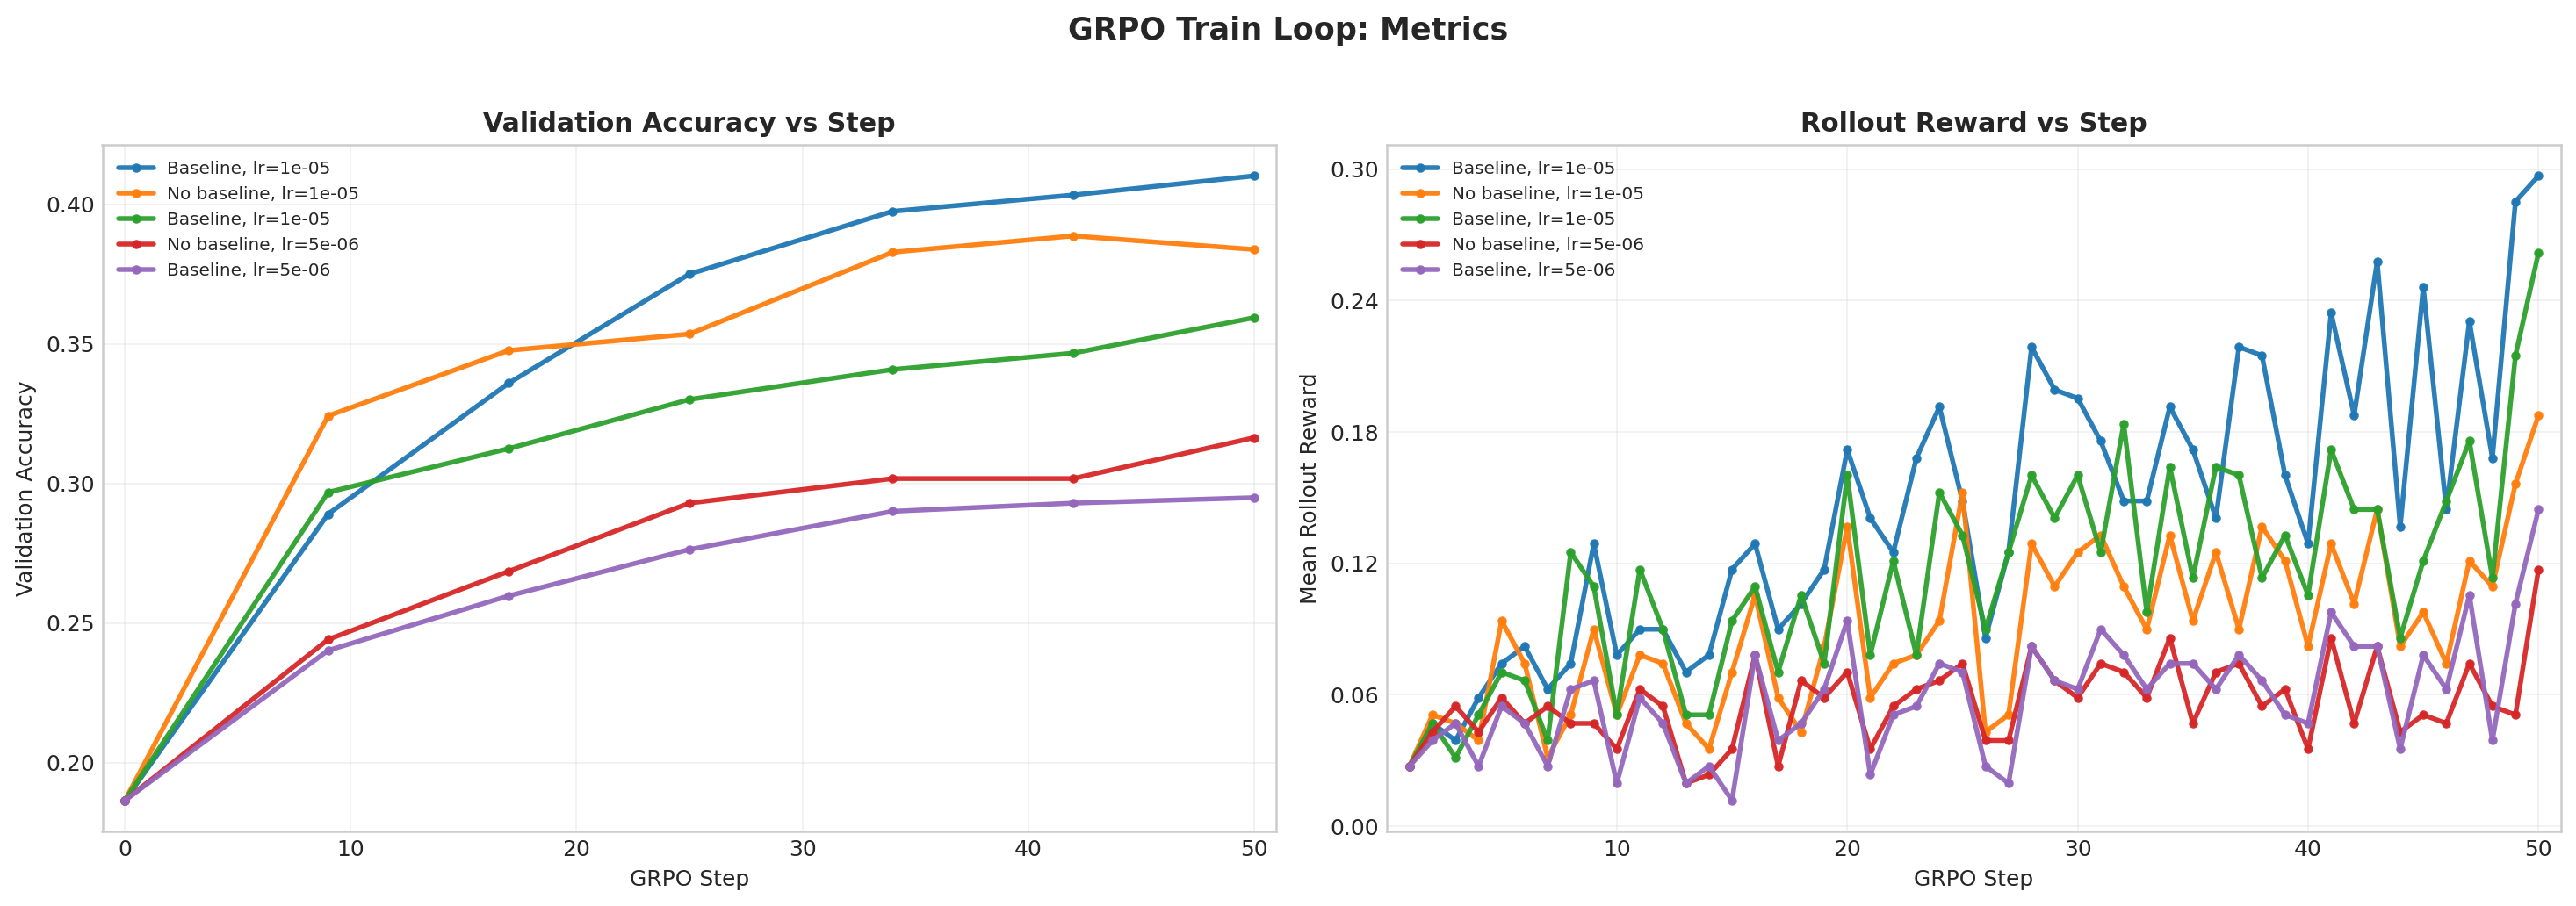
\includegraphics[width=0.8\textwidth]{section7_train_loop.png}
			\caption{Initial GRPO train-loop validation metrics.}
		\end{figure}
		
		\begin{modeloutput}{}
			Question:
			Let $R$ be a unit square region and $n \geq 4$ an integer. A point $X$ in the interior of $R$ is called $n$-ray partitional if there are $n$ rays emanating from $X$ that divide $R$ into $n$ triangles of equal area. How many points are $100$-ray partitional but not $60$-ray partitional?
			$\textbf{(A)}\ 1500 \qquad \textbf{(B)}\ 1560 \qquad \textbf{(C)}\ 2320 \qquad \textbf{(D)}\ 2480 \qquad \textbf{(E)}\ 2500$
			
			Step 0 response excerpt:
			"Let $R$ be a unit square region and $n \geq 4$... The number of points that are $n$-ray partitional is given by the formula $\frac{n^2}{4}$. Therefore, the number of points that are $100$-ray partitional but not $60$-ray partitional is $\frac{100^2}{4} - \frac{60^2}{4} = 2500 - 900 = 1600$. However, we must also consider... total number... is $3200$... we must also consider the intersection... $900$... therefore... $2300$... however... also consider... therefore... $2300$..."
			
			Metrics: format\_reward=0.0, answer\_reward=0.0, reward=0.0, avg\_token\_entropy=0.13367187976837158, response\_length=1024
			
			Step 25 response excerpt:
			"Let $R$ be a unit square region and $n \geq 4$... How many points are $100$-ray partitional but not $60$-ray partitional?</think> <answer>2320</answer>"
			
			Metrics: format\_reward=1.0, answer\_reward=1.0, reward=1.0, avg\_token\_entropy=0.17621006071567535, response\_length=105
			
			Step 50 response excerpt:
			"Let $R$ be a unit square region and $n \geq 4$... How many points are $100$-ray partitional but not $60$-ray partitional?</think> <answer>2320</answer>"
			
			Metrics: format\_reward=1.0, answer\_reward=1.0, reward=1.0, avg\_token\_entropy=0.13026106357574463, response\_length=105
			
		\end{modeloutput}
		
		\textit{Implemented in \repofile{cs336_alignment/section7/grpo_experiment.py}{cs336\_alignment/section7/grpo\_experiment.py}.}
		
	\end{itemize}
	
	\section{GRPO Experiments}
	
	\subsection{Problem (grpo\_learning\_rate): Tune the learning rate}
	
	\begin{itemize}
		\item[(a)] Perform a sweep over the learning rates and report the final validation answer rewards. Provide a model that achieves validation accuracy of at least 25\% on MATH, and briefly discuss other trends in the logged metrics.
		
		The learning-rate sweep showed that \texttt{1e-5} achieved the best performance, reaching 0.3535 validation accuracy, compared to 0.2598 for \texttt{5e-6} and a collapse to 0.0068 for \texttt{3e-5}. Across other metrics, the dominant trend was stability: the \texttt{1e-5} run remained nearly unchanged from its best to final checkpoint, while the higher learning rate exhibited classic divergence, with catastrophic degradation by the end of training.
		
		\begin{figure}[H]
			\centering
			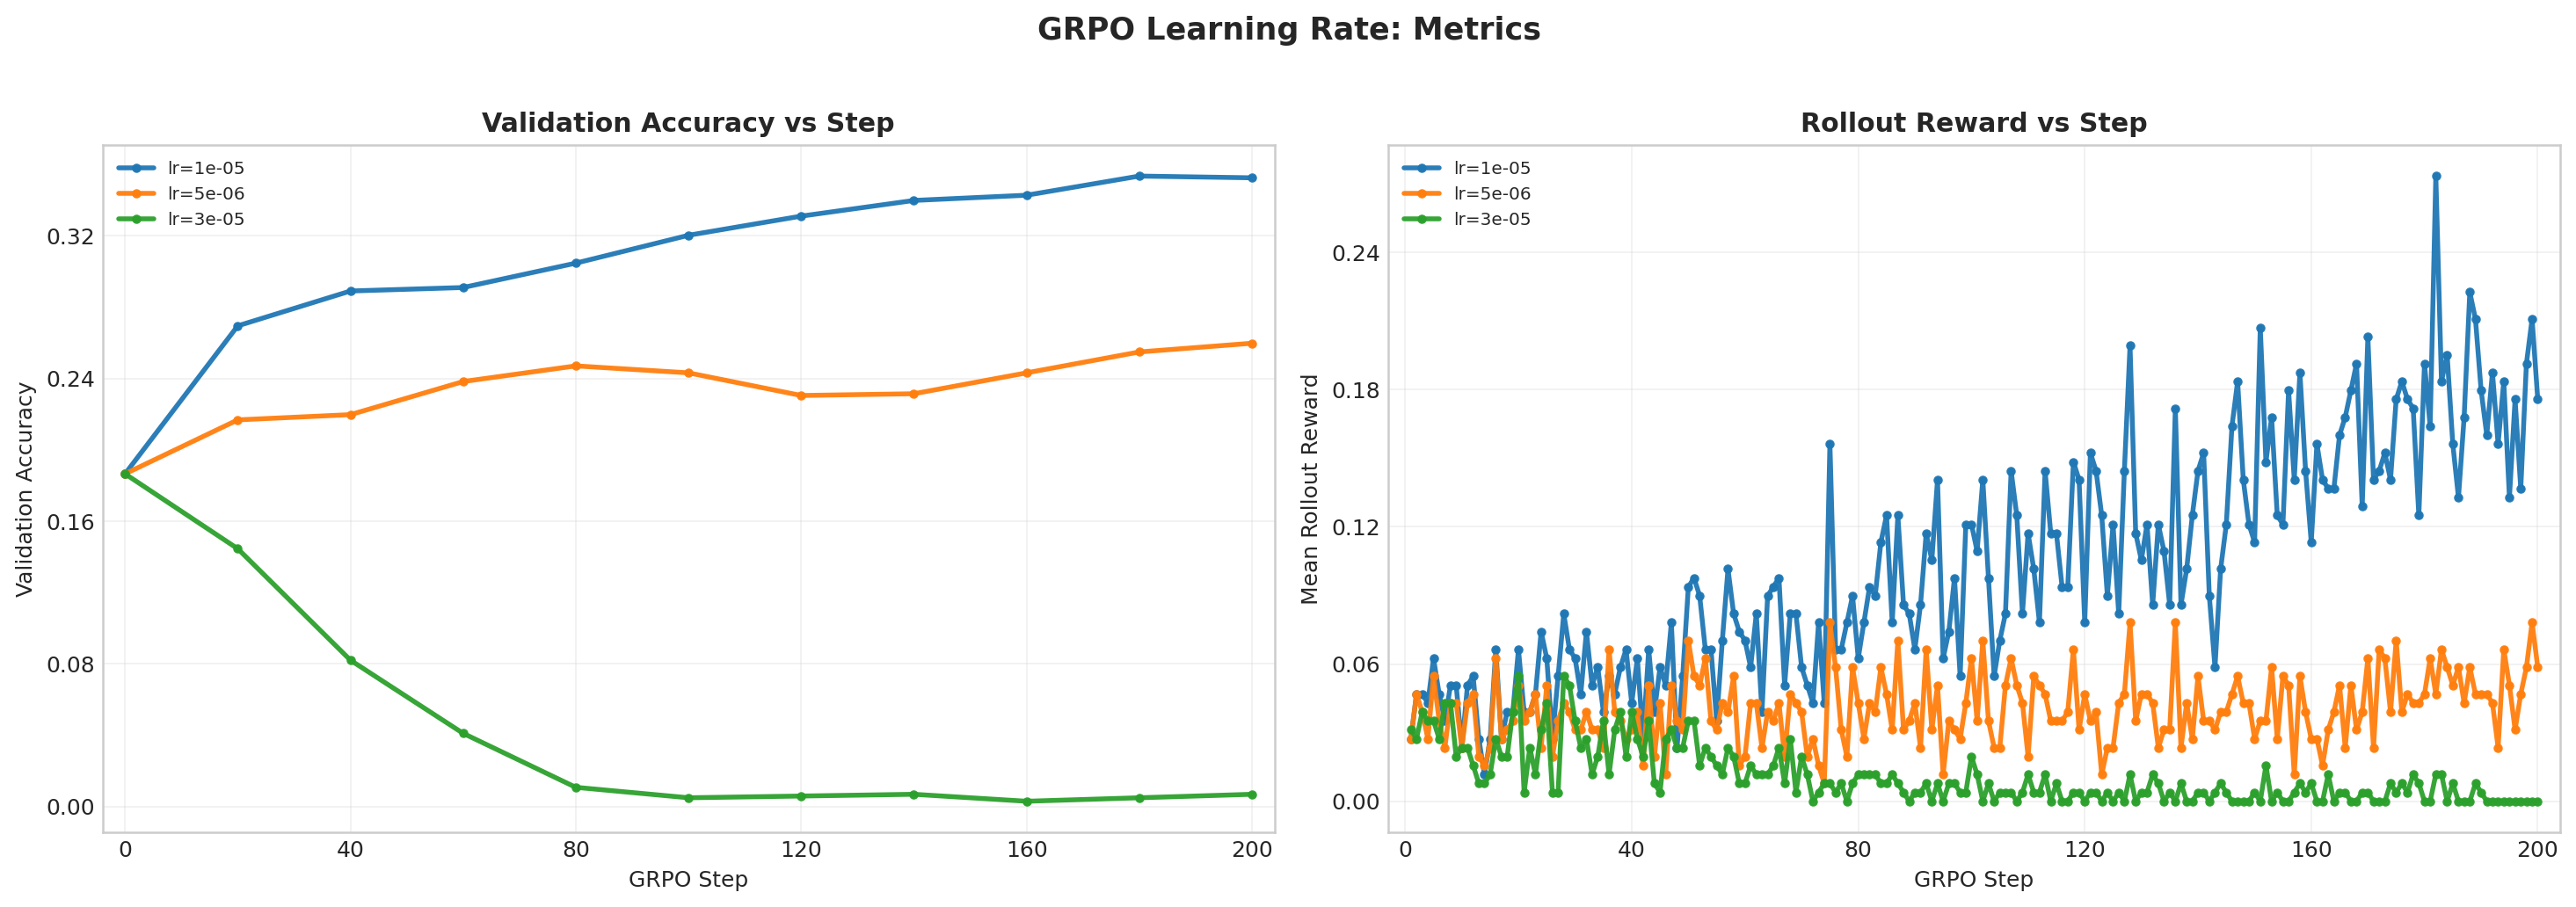
\includegraphics[width=0.8\textwidth]{section7_learning_rate.png}
			\caption{Validation metrics for the GRPO learning-rate sweep.}
		\end{figure}
		
	\end{itemize}
	
	\subsection{Problem (grpo\_baselines): Effect of baselining}
	
	\begin{itemize}
		\item[(a)] Train a policy with \texttt{reinforce\_with\_baseline} and with \texttt{no\_baseline}. Report the validation reward curves and comment on other trends.
		
		In this artifact slice, \texttt{no\_baseline} unexpectedly outperformed \texttt{reinforce\_with\_baseline}, reaching 0.3545 versus 0.3164 validation accuracy. The reward traces show that the baseline variant achieved a slightly higher peak rollout reward, but that did not translate into better validation accuracy, which suggests that the control-variate benefit here was offset by worse optimization dynamics for the actual answer metric.
		
		\begin{figure}[H]
			\centering
			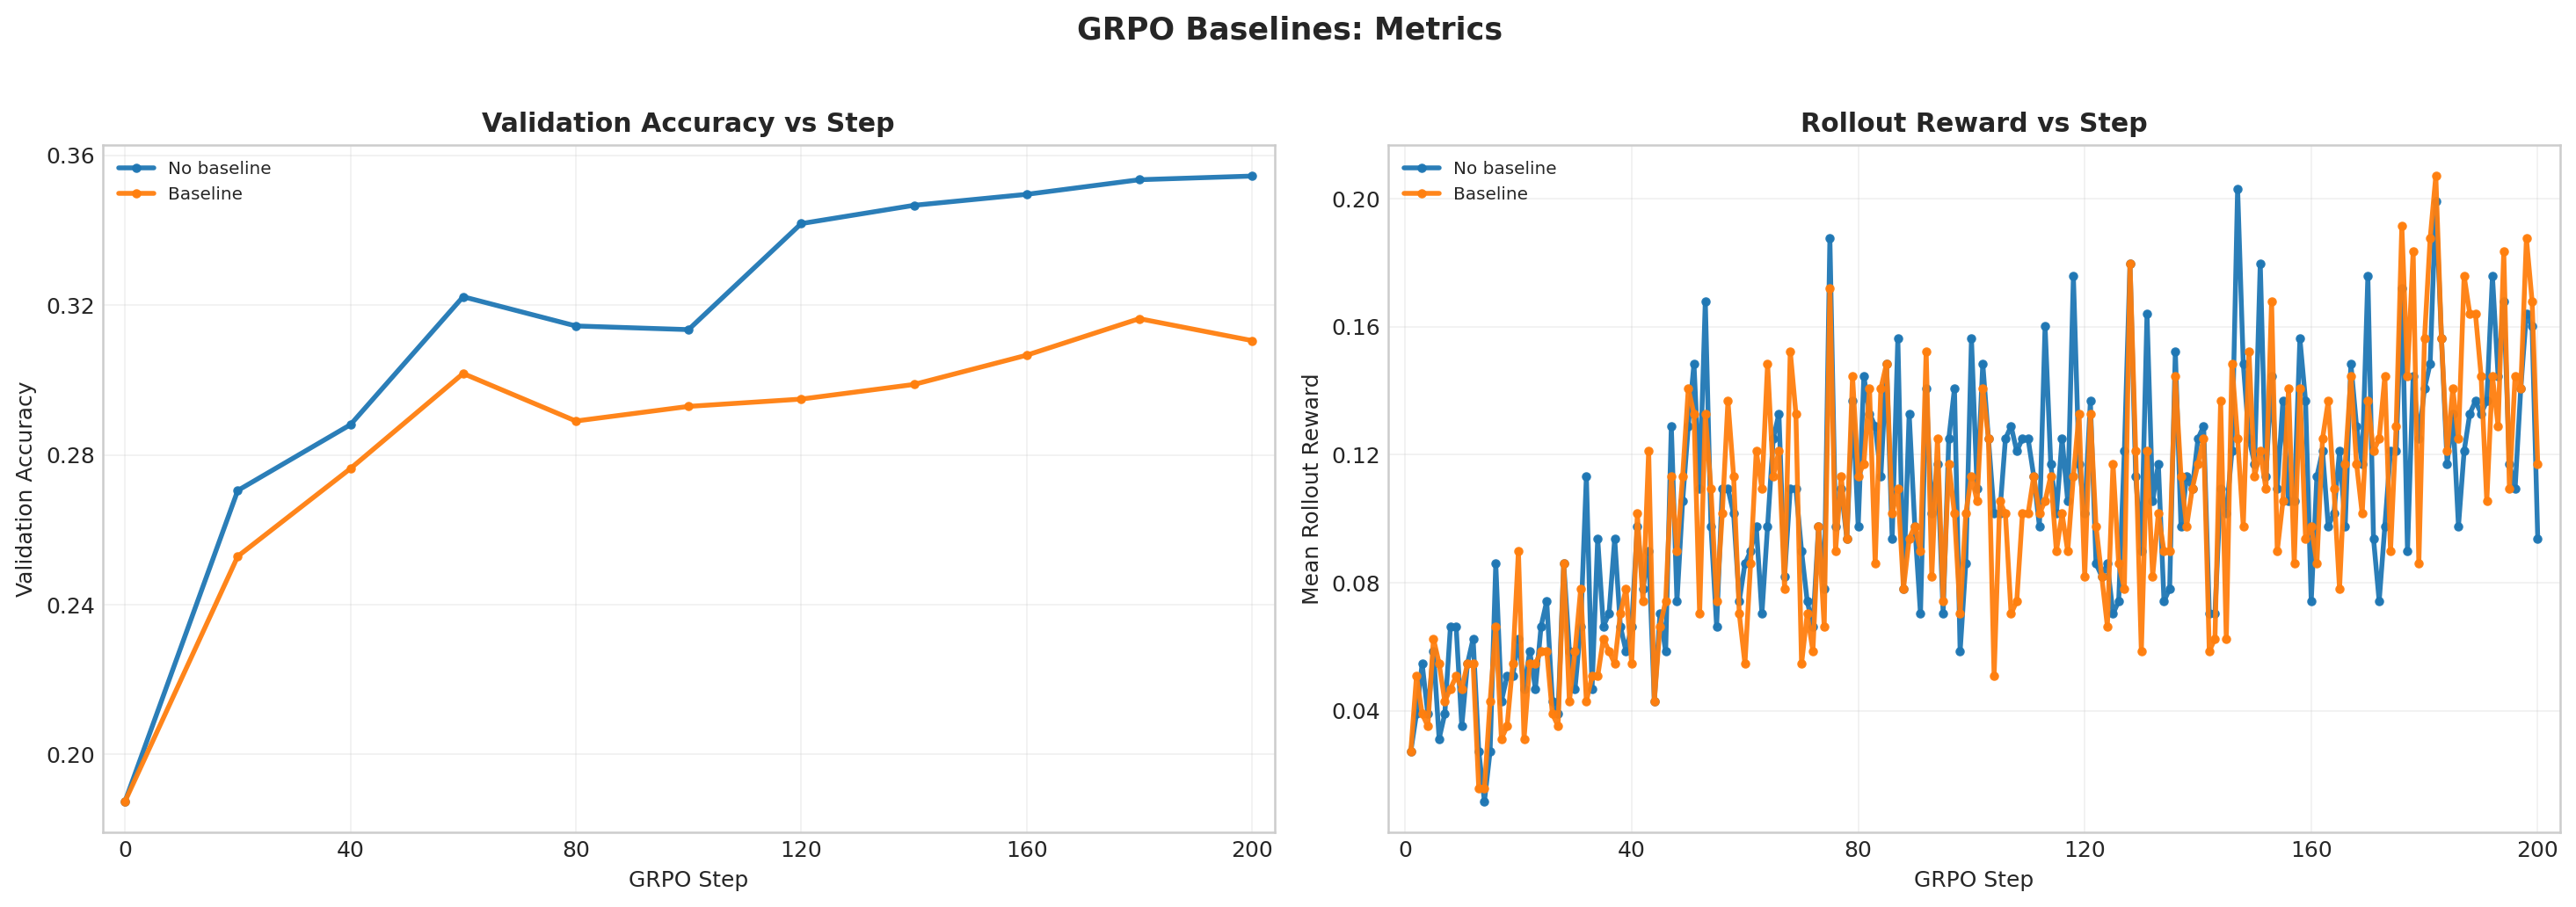
\includegraphics[width=0.8\textwidth]{section7_baselines.png}
			\caption{Validation metrics for the baselining ablation.}
		\end{figure}
		
	\end{itemize}
	
	
	\subsection{Problem (think\_about\_length\_normalization): Think about length normalization}
	
	\begin{itemize}
		\item[(a)] Compare the two approaches (without running experiments yet). What are the pros and cons of each approach? Are there any specific settings or examples where one approach seems better?
		
		\texttt{masked\_mean} averages each response by its own generated length, so each example contributes roughly equally regardless of response length. This is appealing when the goal is to avoid overweighting verbose samples, but it also means that shorter responses receive larger per-token gradients than longer responses.
		
		In contrast, \texttt{masked\_normalize} divides by a fixed constant, which preserves equal per-token weight across responses and matches the intuition that each sampled action should contribute comparably; the tradeoff is that very short responses no longer get their loss normalized to the same per-example scale.
		
		For reasoning RL, the fixed-constant approach seemed more principled because it avoids implicitly rewarding brevity through larger per-token updates on short responses. That makes \texttt{masked\_normalize} especially attractive when response lengths vary widely or when long solutions are often necessary for correctness.
		
	\end{itemize}
	
	\subsection{Problem (grpo\_length\_normalization): Effect of length normalization}
	
	\begin{itemize}
		\item[(a)] Compare normalization with \texttt{masked\_mean} and \texttt{masked\_normalize} with an end-to-end GRPO training run. Report the validation answer reward curves and comment on the findings.
		
		The empirical comparison slightly favors fixed-constant normalization: \texttt{masked\_normalize} achieves 0.3066 validation accuracy versus 0.2910 for \texttt{masked\_mean}. While the gap is modest, it is consistent with the theoretical expectation that fixed normalization provides more uniform token-level credit assignment across short and long completions.
		
		A clearer secondary effect appears in gradient stability. During GRPO training,  \texttt{masked\_mean} produces larger and more variable updates, with mean gradient norm 0.0061, standard deviation 0.0092, and peak 0.0405. In contrast, \texttt{masked\_normalize} reduces these to 0.0011, 0.0015, and 0.0054, respectively. Thus, the fixed-constant variant not only improves validation accuracy slightly but also yields significantly smoother optimization dynamics.
		
		It also produces slightly longer responses on average (846 vs.\ 822 tokens per training step), consistent with the idea that normalization by response length can implicitly bias update magnitudes toward shorter completions.
		
		\begin{figure}[H]
			\centering
			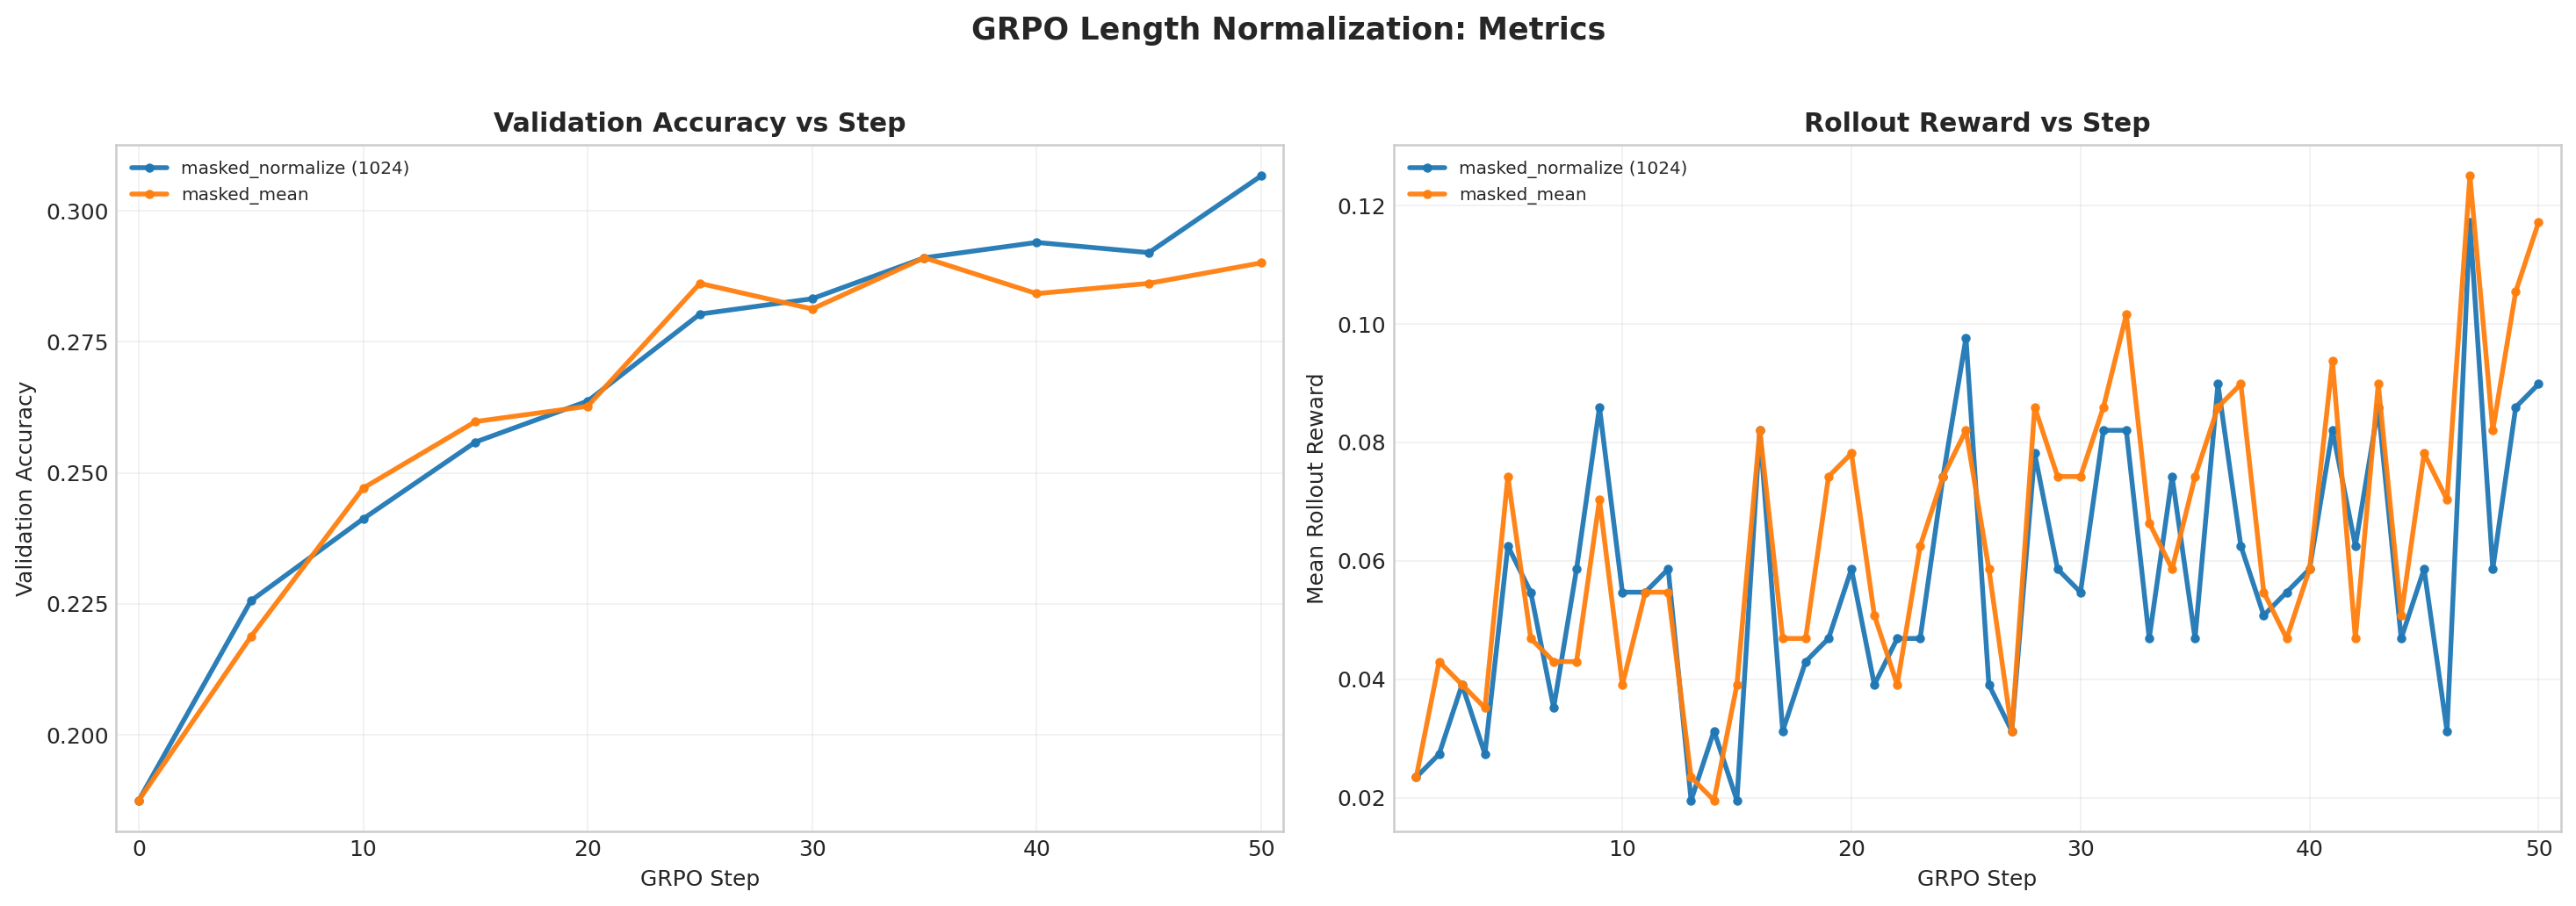
\includegraphics[width=0.8\textwidth]{section7_length_normalization.png}
			\caption{Validation metrics for length-normalization variants.}
		\end{figure}
		
	\end{itemize}
	
	\subsection{Problem (grpo\_group\_standard\_deviation): Effect of standard deviation normalization}
	
	\begin{itemize}
		\item[(a)] Compare the performance of \texttt{use\_std\_normalization == True} and \texttt{use\_std\_normalization == False}. Report the validation answer reward curves and comment on the findings.
		
		Removing standard-deviation normalization yields a small gain: \texttt{use\_std\_normalization = False} reaches 0.3125 validation accuracy versus 0.3086 with normalization enabled. While modest, this difference is consistent with the hypothesis that per-group standard deviation scaling can distort the relative strength of updates across questions.
		
		The stability picture is more nuanced. The no-std run exhibits larger early gradient variability, with mean gradient norm 0.0074 (vs.\ 0.0065), standard deviation 0.0113 (vs.\ 0.0084), and peak 0.0520 (vs.\ 0.0383). However, later-stage updates are smaller without normalization (0.0078 vs.\ 0.0126), and the run ultimately achieves slightly higher validation accuracy and rollout reward. This suggests that while std normalization reduces gradient spikes, it may also over-dampen high-impact updates.
		
		The no-std variant also produces slightly shorter responses on average (810 vs.\ 826 tokens per step), indicating that the main effect is in update weighting rather than a meaningful change in generation style.
		
		\begin{figure}[H]
			\centering
			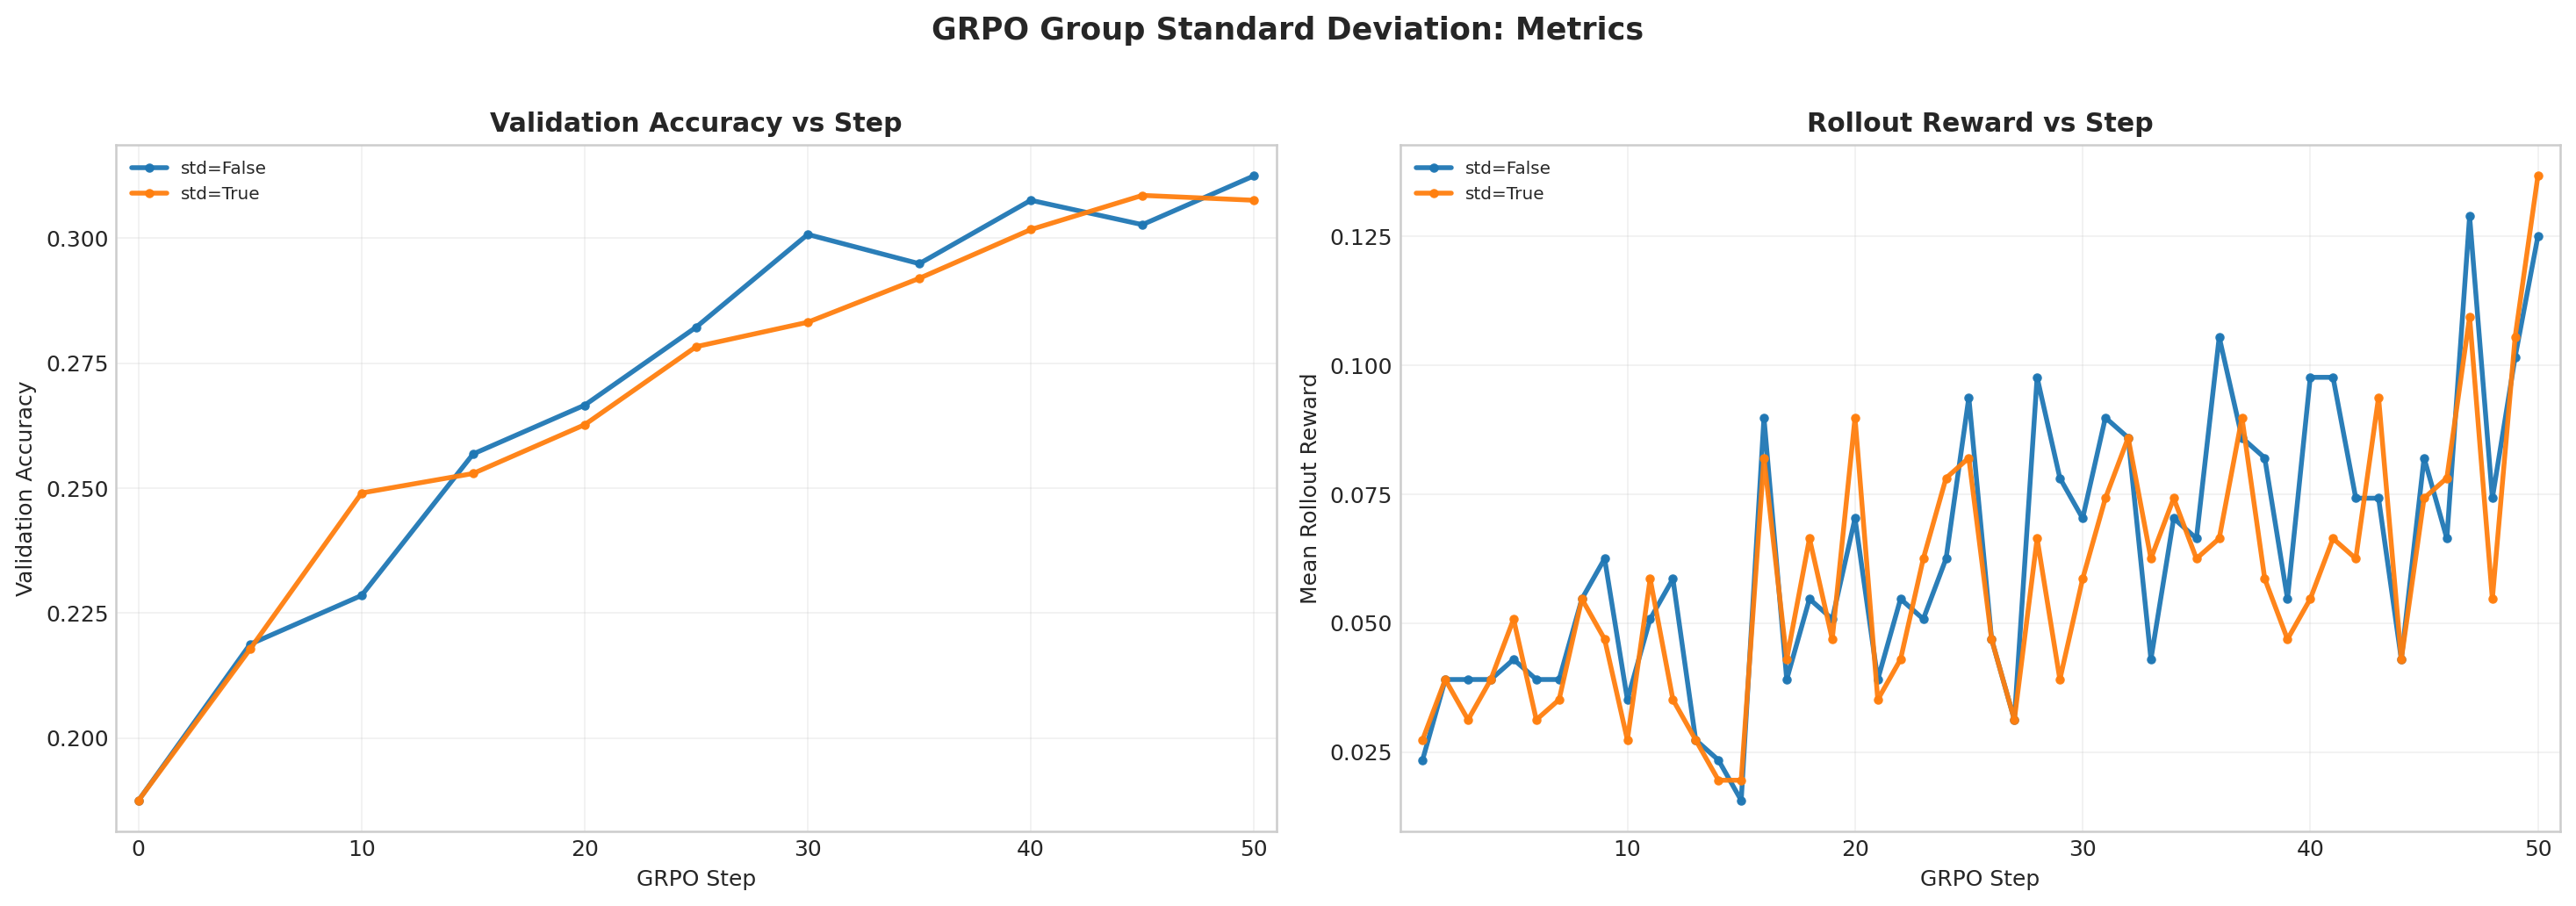
\includegraphics[width=0.8\textwidth]{section7_group_std.png}
			\caption{Validation metrics for group-standard-deviation normalization.}
		\end{figure}
		
	\end{itemize}
	
	\subsection{Problem (grpo\_off\_policy): Implement off-policy GRPO}
	
	\begin{itemize}
		\item[(a)] Implement off-policy GRPO training.
		
		\textit{Implemented in \repofile{cs336_alignment/section7/grpo_experiment.py}{cs336\_alignment/section7/grpo\_experiment.py}.}
		
	\end{itemize}
	
	\subsection{Problem (grpo\_off\_policy\_sweep): Off-policy GRPO hyperparameter sweep}
	
	\begin{itemize}
		\item[(a)] Fixing \texttt{rollout\_batch\_size = 256}, choose a range over \texttt{epochs\_per\_rollout\_batch} and \texttt{train\_batch\_size} to sweep over. First do a broad sweep for a limited number of GRPO steps, then a more focused sweep for a larger number of steps. Provide a brief experiment log explaining the chosen ranges, and compare to the on-policy run using validation curves and wall-clock time.
		
		The broad sweep used four settings that keep the rollout batch fixed at 256 while increasing the number of optimizer passes over the same rollout data: \texttt{(epochs, train\_batch) = (1,256), (2,128), (4,128), (8,64)}. This range was chosen to span the on-policy baseline, a mild off-policy regime, and two progressively more aggressive reuse regimes.
		
		In the broad sweep, more reuse helped up to a point: the 8-epoch clipped run reached the best validation accuracy at 0.3721, beating the on-policy 1-epoch baseline at 0.2656 in the same broad comparison. The wall-clock view also showed the expected cost tradeoff, with the most accurate run taking 77.5 minutes versus 15.5 minutes for the fastest baseline.
		
		\begin{figure}[H]
			\centering
			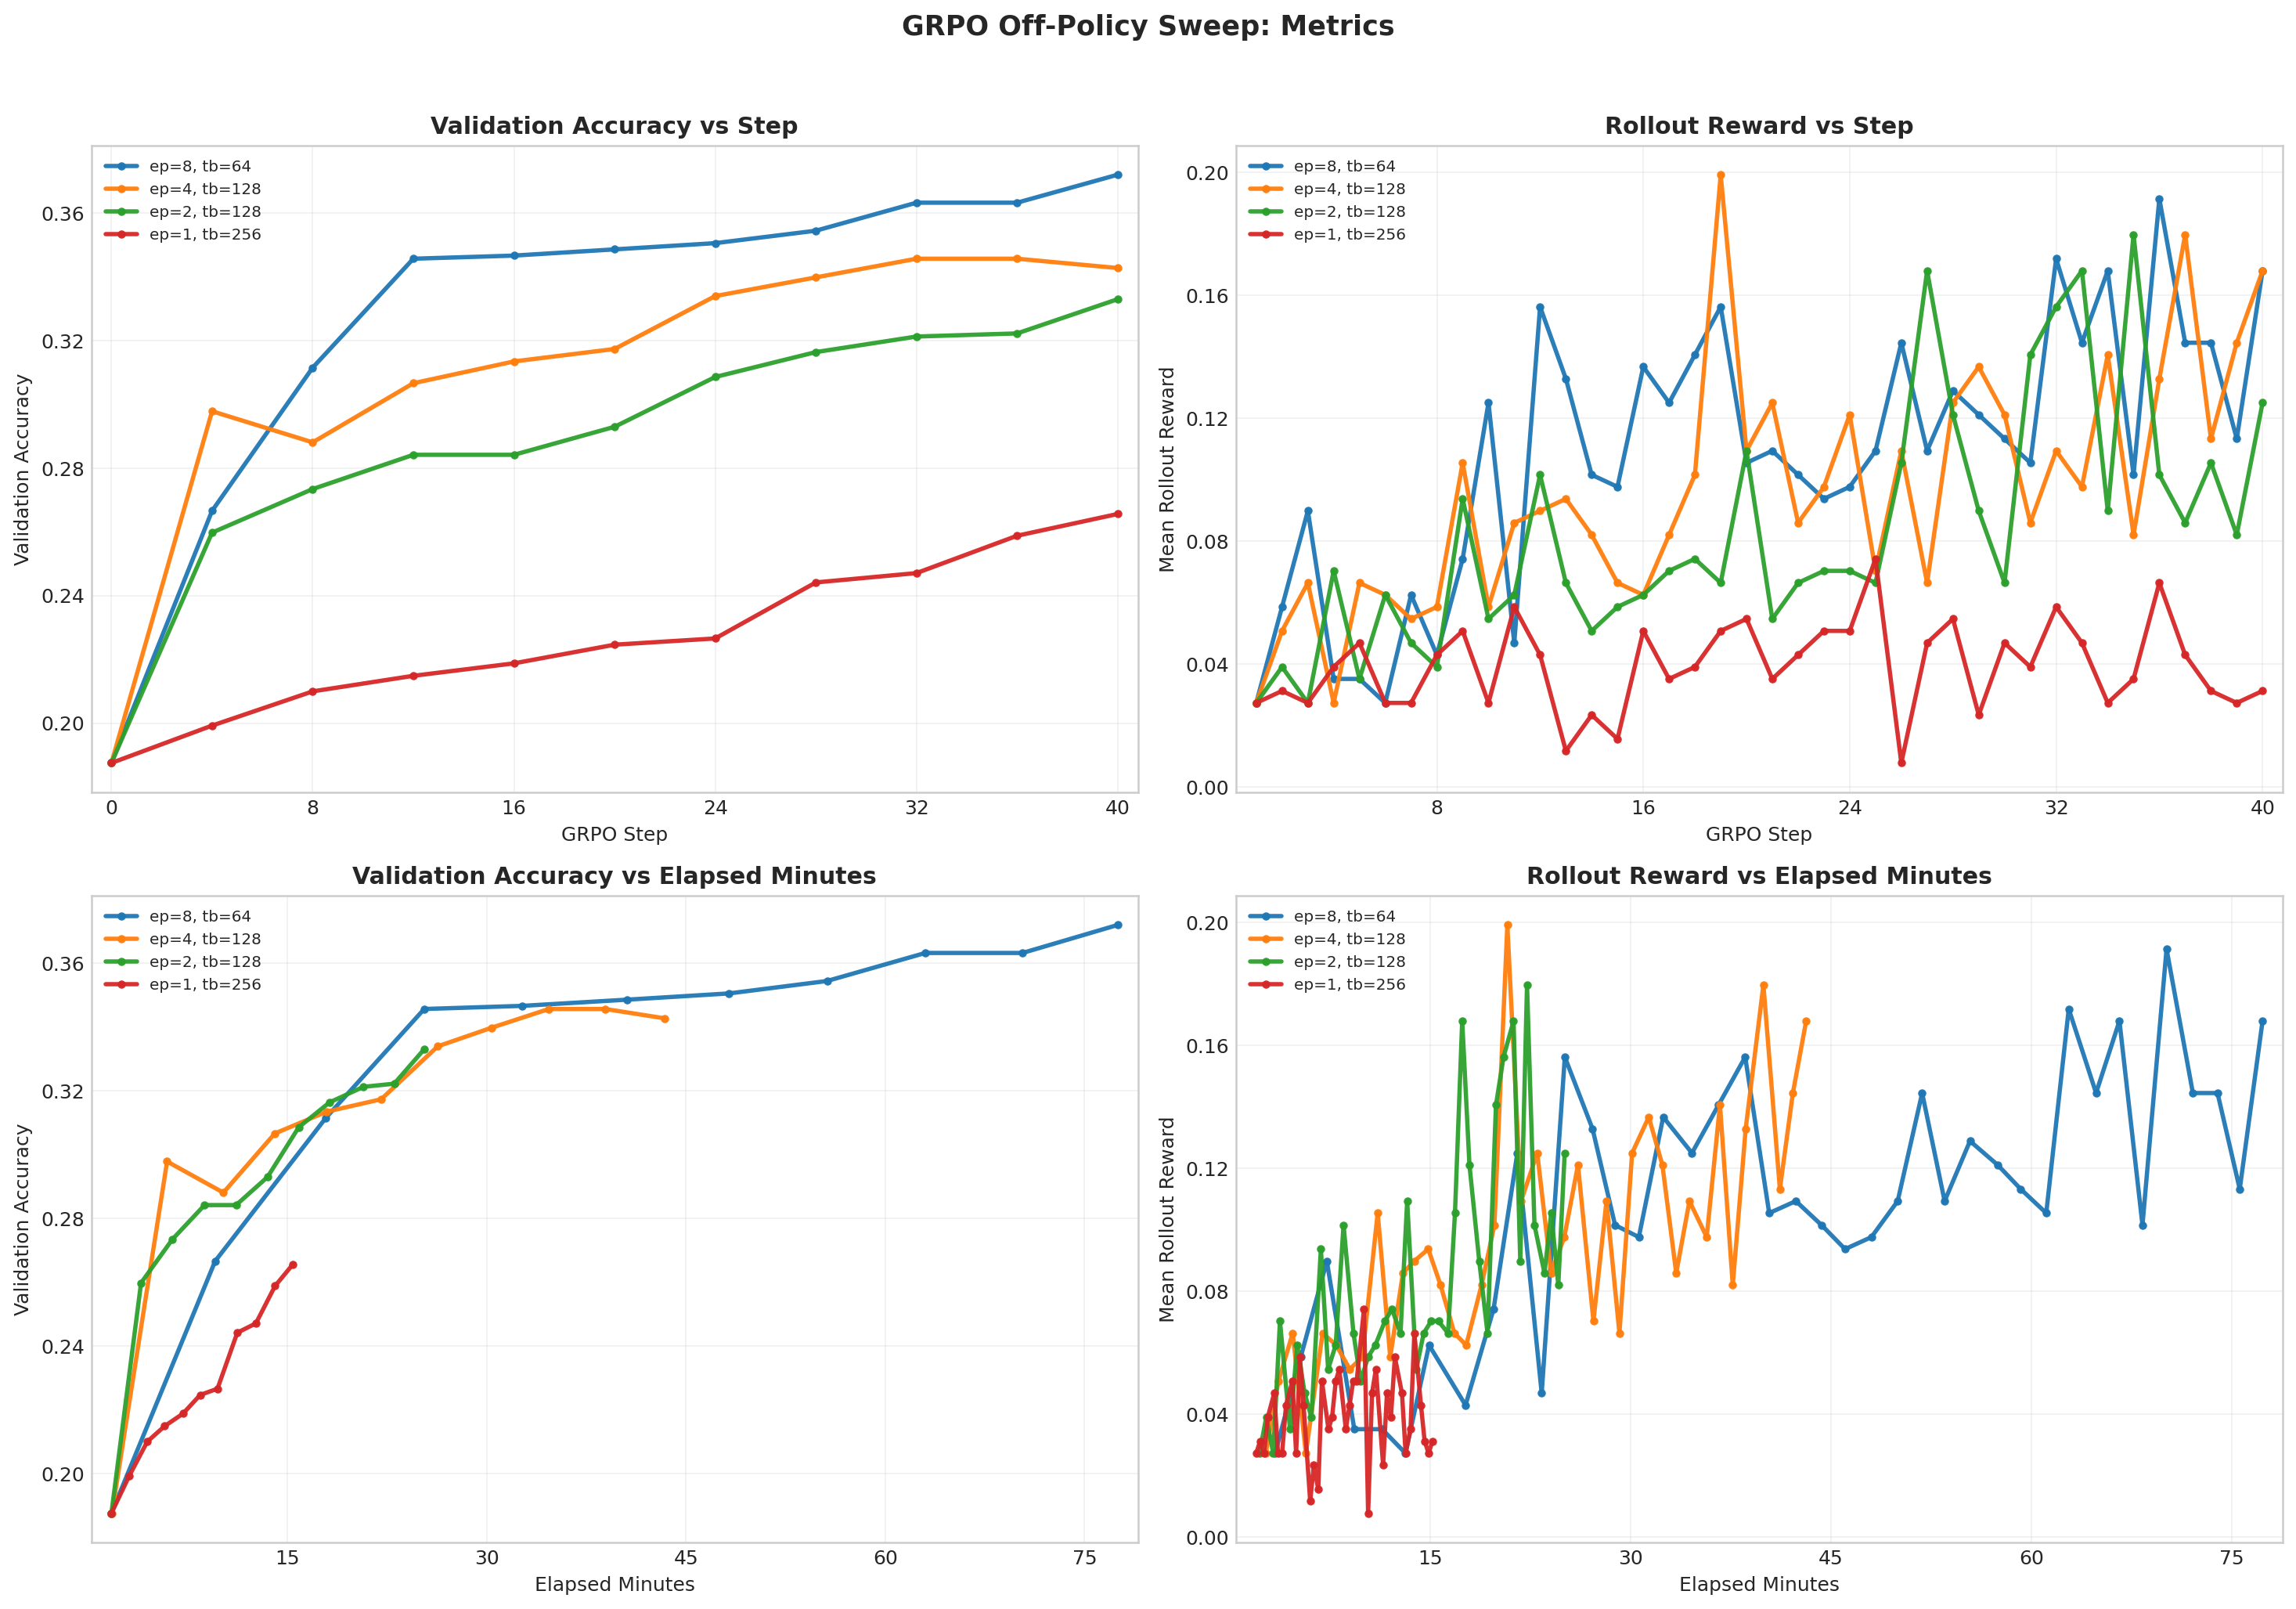
\includegraphics[width=0.8\textwidth]{section7_off_policy_broad.png}
			\caption{Broad off-policy GRPO sweep, including the wall-clock comparison.}
		\end{figure}
		
		In the focused sweep, results are less consistent. A simpler 1-epoch \texttt{no\_baseline} configuration reaches 0.3535 validation accuracy, outperforming the more heavily reused clipped variants. This breaks the monotonic trend observed in the broad sweep, suggesting sensitivity to optimization details at higher reuse levels.
		
		\begin{figure}[H]
			\centering
			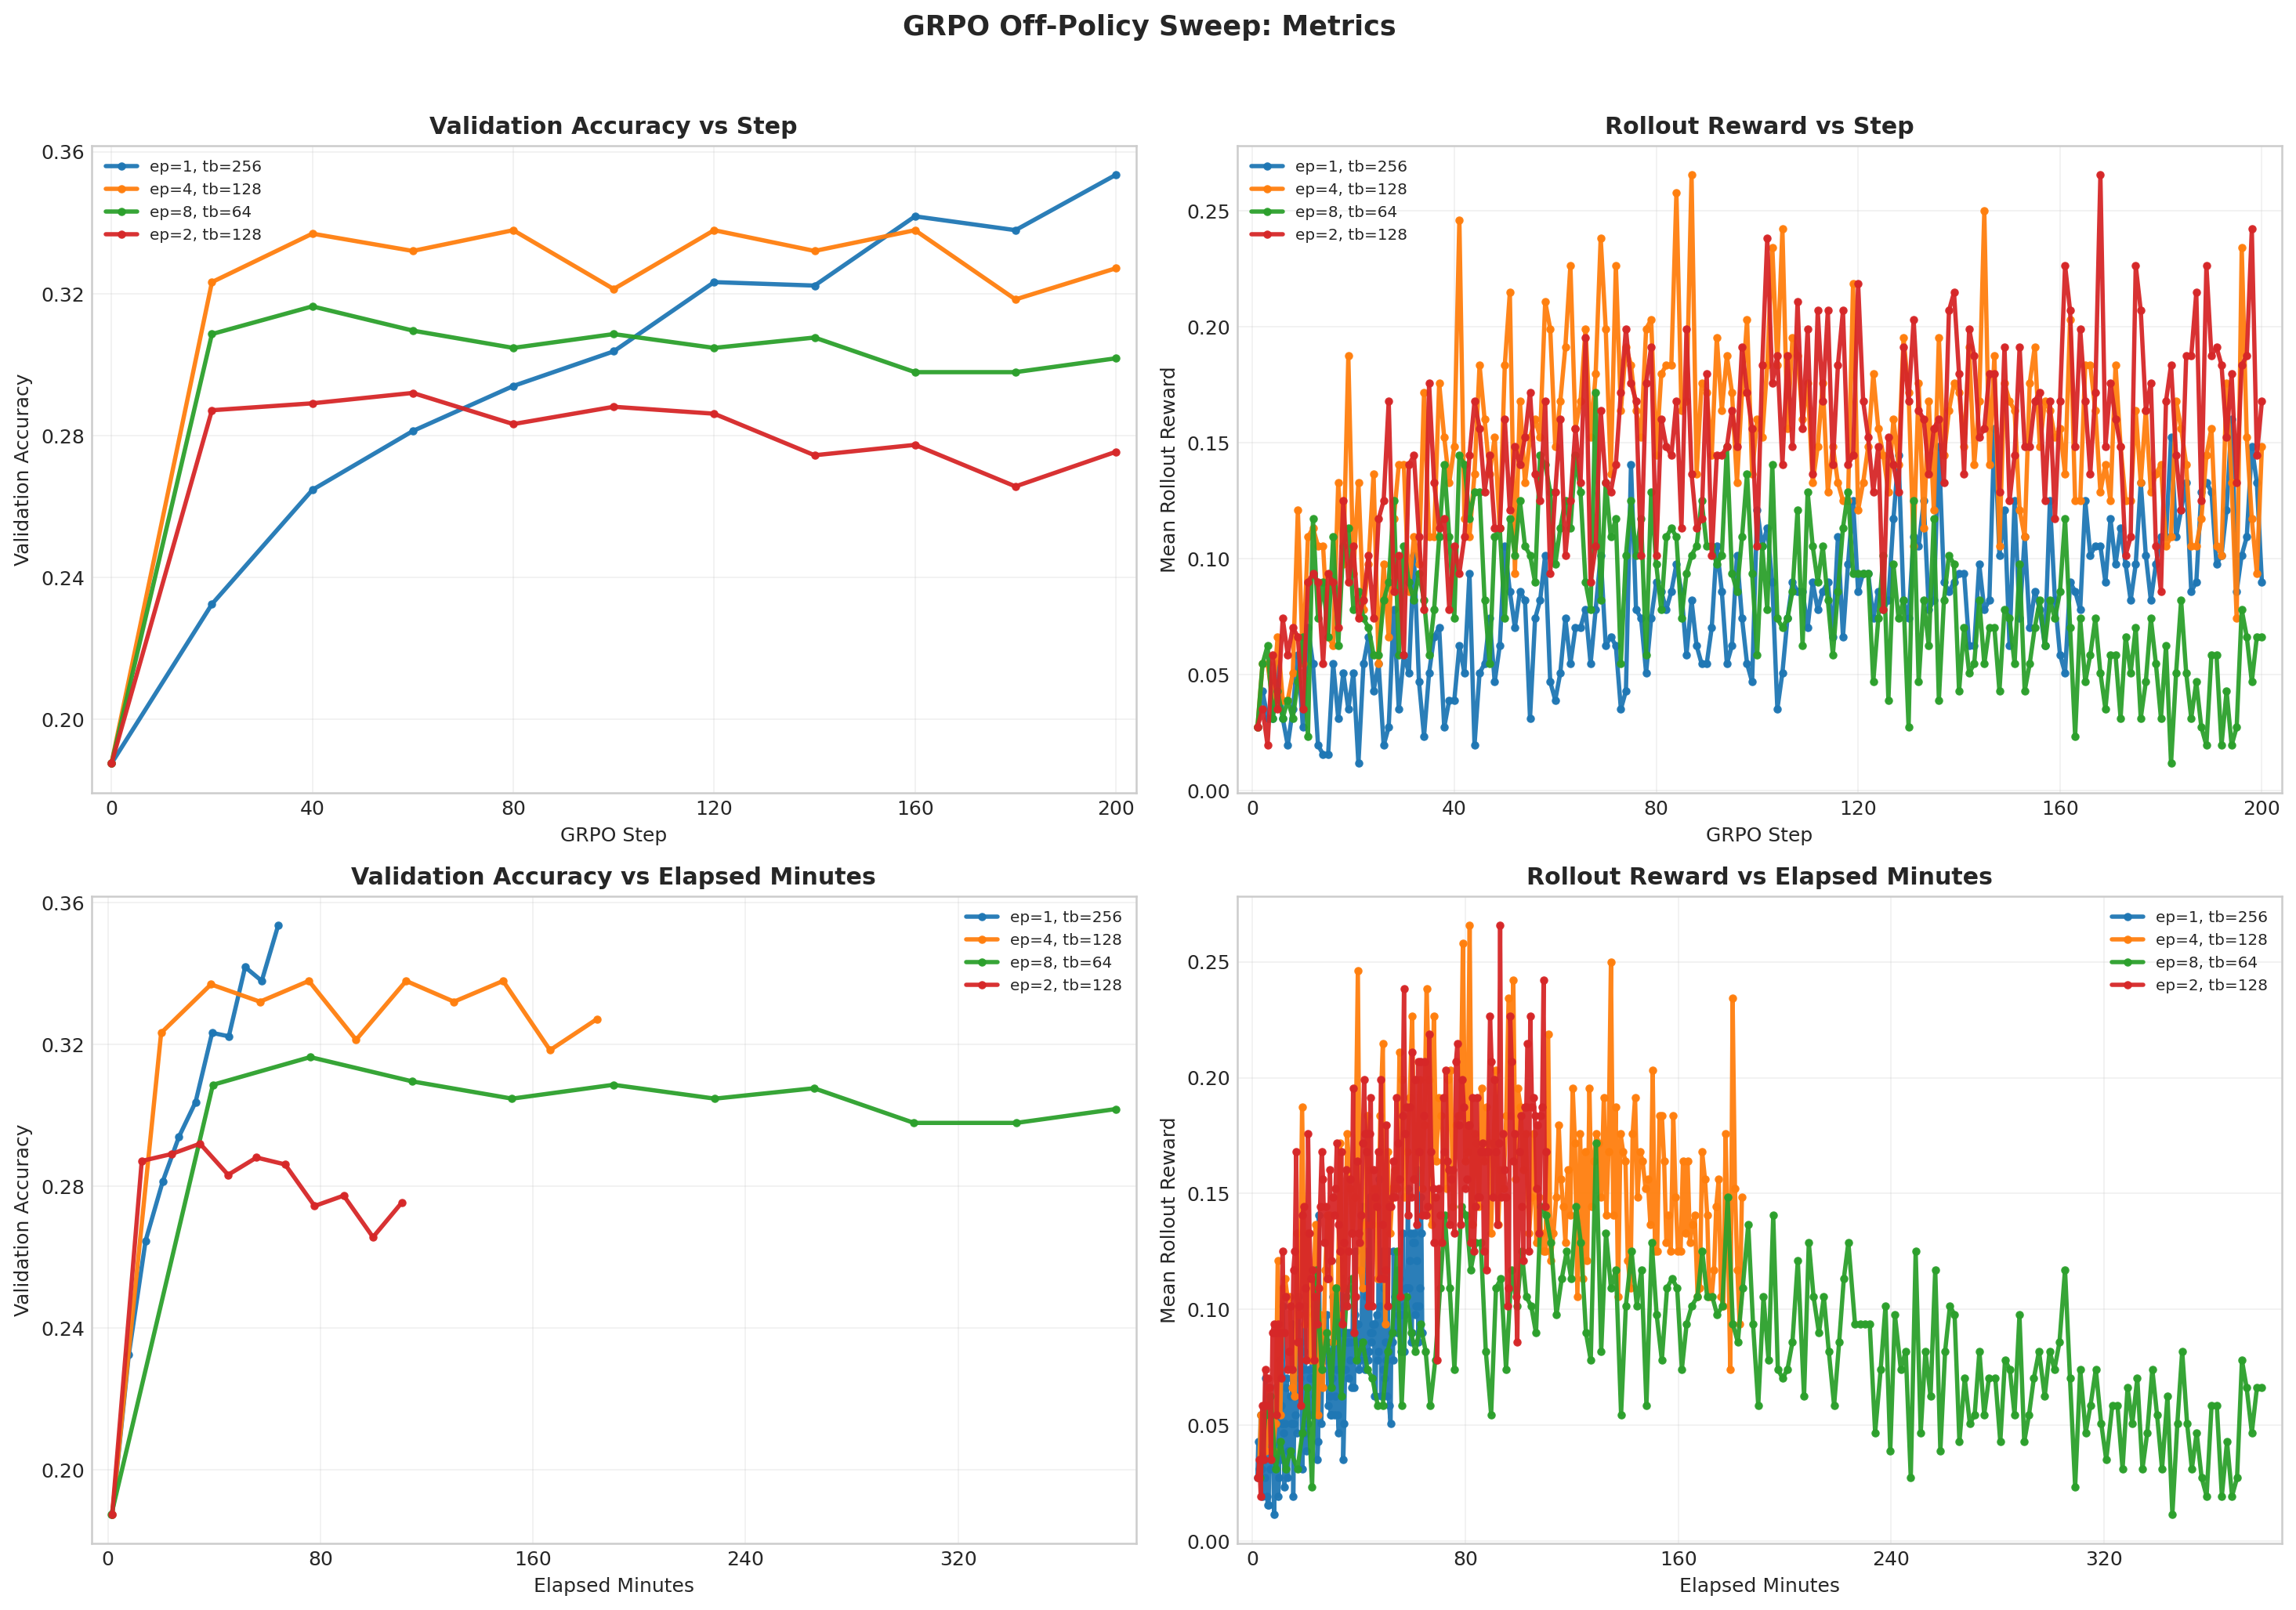
\includegraphics[width=0.8\textwidth]{section7_off_policy_focused.png}
			\caption{Focused off-policy GRPO sweep.}
		\end{figure}
		
		The overall conclusion is that off-policy reuse can improve sample efficiency, but the more aggressive settings are sensitive and do not guarantee a better accuracy-time tradeoff in every run.
		
	\end{itemize}
	
	\subsection{Problem (grpo\_off\_policy\_clip\_ablation): Off-policy GRPO-Clip ablation}
	
	\begin{itemize}
		\item[(a)] Implement the unclipped per-token loss as a new loss type \texttt{GRPO-No-Clip}. Take your best performing off-policy hyperparameters and run the unclipped version of the loss. Report the validation answer reward curves and comment on the findings.
		
		The unclipped objective is markedly less stable. Although \texttt{grpo\_no\_clip} achieves a nontrivial peak validation accuracy of 0.3242, it subsequently collapses to 0.0000 final accuracy. In contrast, the clipped variant peaks at 0.3613 and retains 0.3213 at the end of training. This behavior aligns with the intended role of clipping: when multiple gradient updates are performed on stale rollout data, constraining the policy ratio becomes critical for maintaining stability.
		
		The auxiliary metrics further highlight this divergence. While the clipped run already exhibits large updates (mean gradient norm 1218.8, peak 962{,}560), it remains numerically stable and continues to produce nonzero reward. In contrast, the unclipped run becomes numerically pathological: gradient norms explode to a mean of approximately $9.2 \times 10^{13}$ and a peak of $9.34 \times 10^{16}$, with 587 out of 1,600 training steps producing non-finite gradients.
		
		Entropy collapses in both settings late in training, but the effect is significantly more severe without clipping. In the unclipped case, near-zero entropy coincides with complete reward collapse and degenerate behavior, including responses saturating the maximum generation length (final mean response length 1024.0 tokens, compared to 659.5 for the clipped run). Overall, relative to \texttt{grpo\_no\_clip}, the unclipped objective is not merely less performant but enters a numerically unstable regime consistent with severe off-policy over-optimization.
		
		\begin{figure}[H]
			\centering
			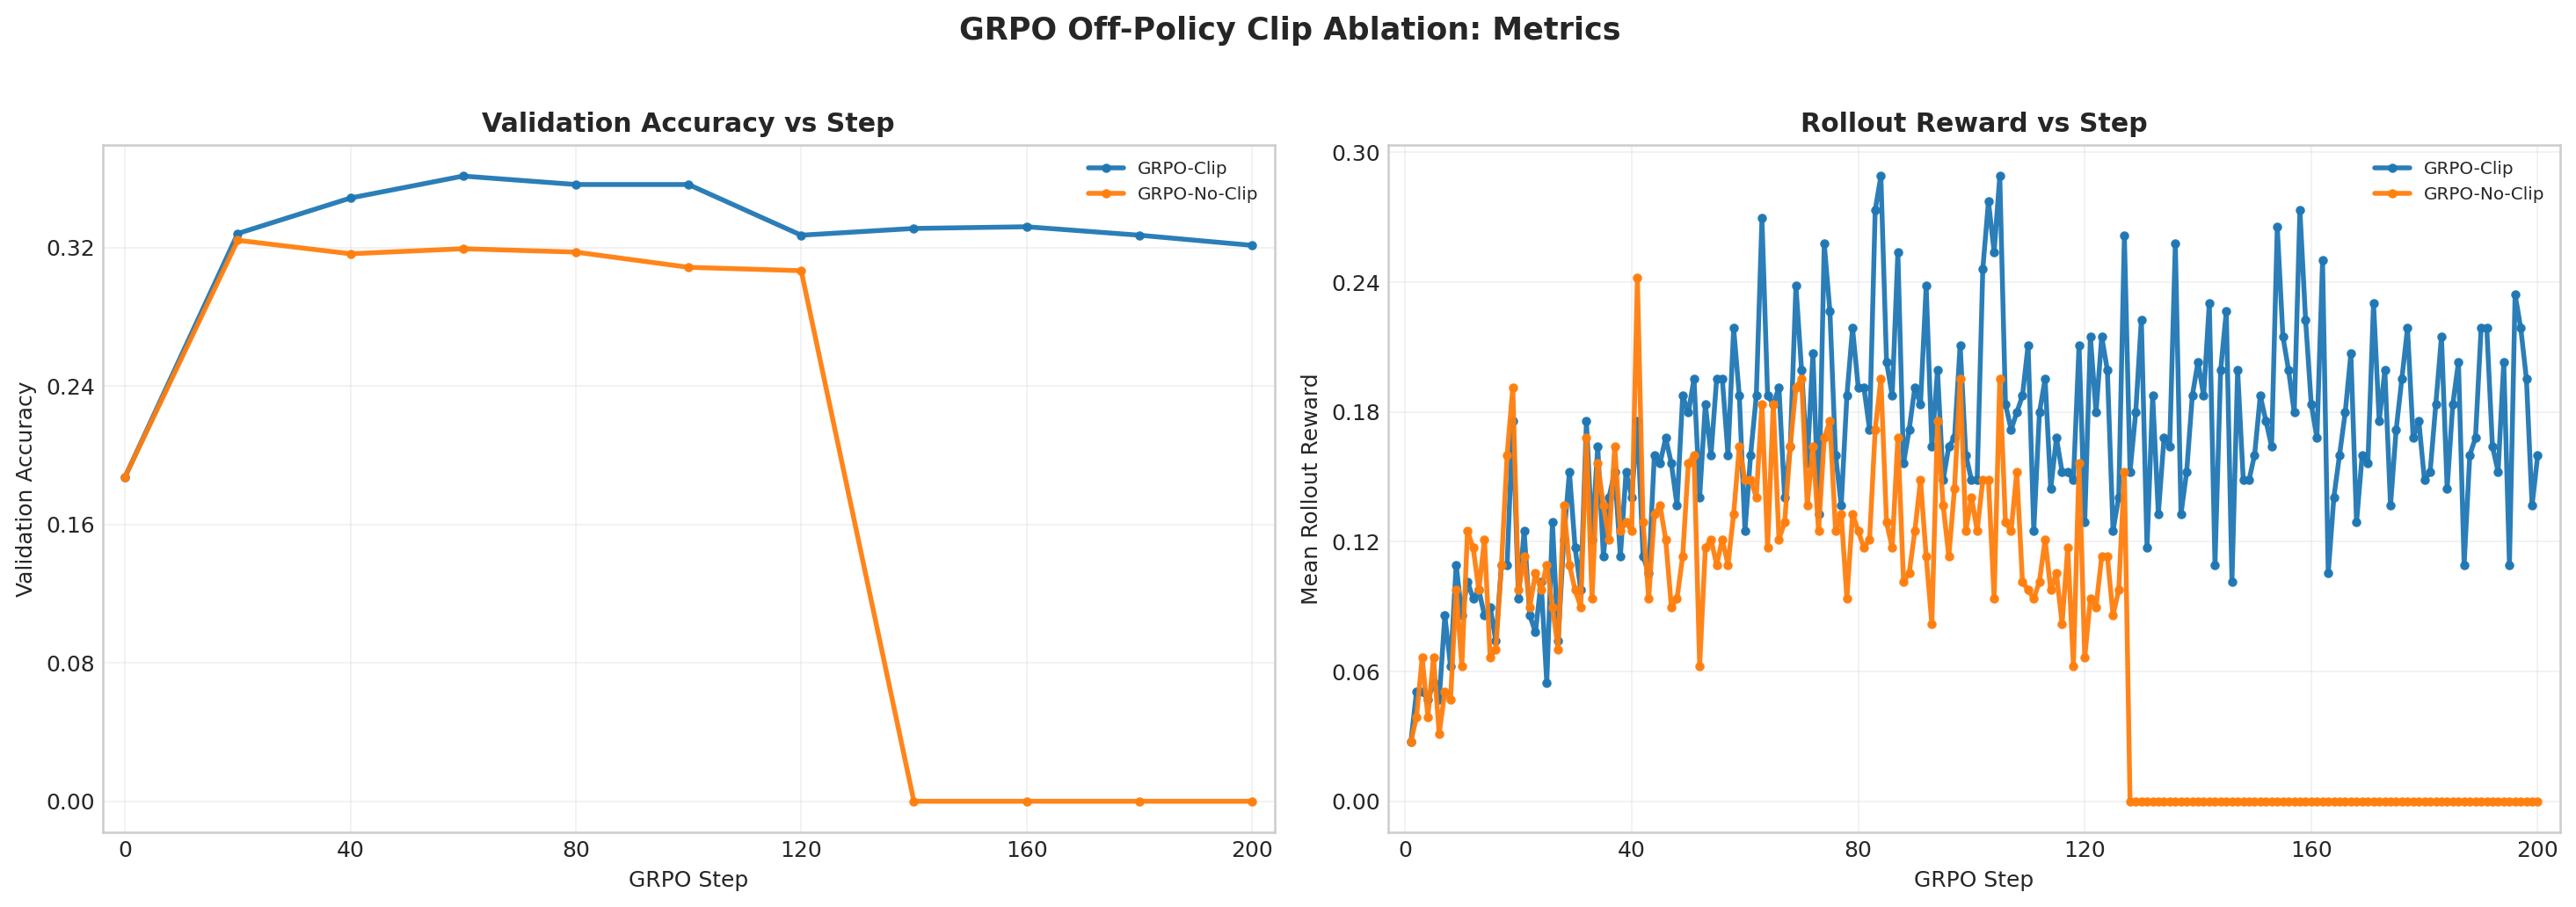
\includegraphics[width=0.8\textwidth]{section7_off_policy_clip_ablation.png}
			\caption{Clipped versus unclipped off-policy GRPO.}
		\end{figure}
		
		\textit{Implemented in  \repofile{cs336_alignment/section7/compute_grpo_no_clip_loss.py}{cs336\_alignment/section7/compute\_grpo\_no\_clip\_loss.py}.}
		
	\end{itemize}
	
	\subsection{Problem (grpo\_prompt\_ablation): Prompt ablation}
	
	\begin{itemize}
		\item[(a)] Report the validation answer reward curves for both the R1-Zero prompt and the question-only prompt. How do metrics compare, including any other metrics that have a noticeable trend such as entropy, response length, and gradient norm? Try to explain your findings.
		
		The prompt ablation produced the strongest result: the question-only setup reached 0.6836 validation accuracy versus 0.3594 for the R1-Zero prompt, a gain of 0.3242. The question-only model also generated much longer responses on average (1547.7 versus 663.6 tokens), which is consistent with the hypothesis in the assignment text that Qwen 2.5 Math 1.5B is better matched to direct question-answer prompting than to the synthetic R1-Zero conversational scaffold.
		
		The other metrics moved just as strongly. The question-only run had far smaller and more stable gradients, with mean gradient norm 0.0222 and peak 0.0625, whereas the R1-Zero run had mean gradient norm 722.3 and peak 405{,}504. Token entropy was also much lower for question-only (mean 0.0606 versus 0.2153), while its final-10-step mean rollout reward was dramatically higher (0.5078 versus 0.1633). Taken together, these metrics suggest that the question-only prompt is not merely eliciting longer outputs; it is producing a much better-conditioned optimization problem, where the model can improve reward without the enormous gradient spikes seen under the R1-Zero scaffold.
		
		This was also the clearest example of prompt choice dominating smaller algorithmic tweaks. Even after substantial work on baselines, normalization, and off-policy training, simply switching to the prompt style better aligned with pretraining moved the accuracy far more than the other ablations.
		
		\begin{figure}[H]
			\centering
			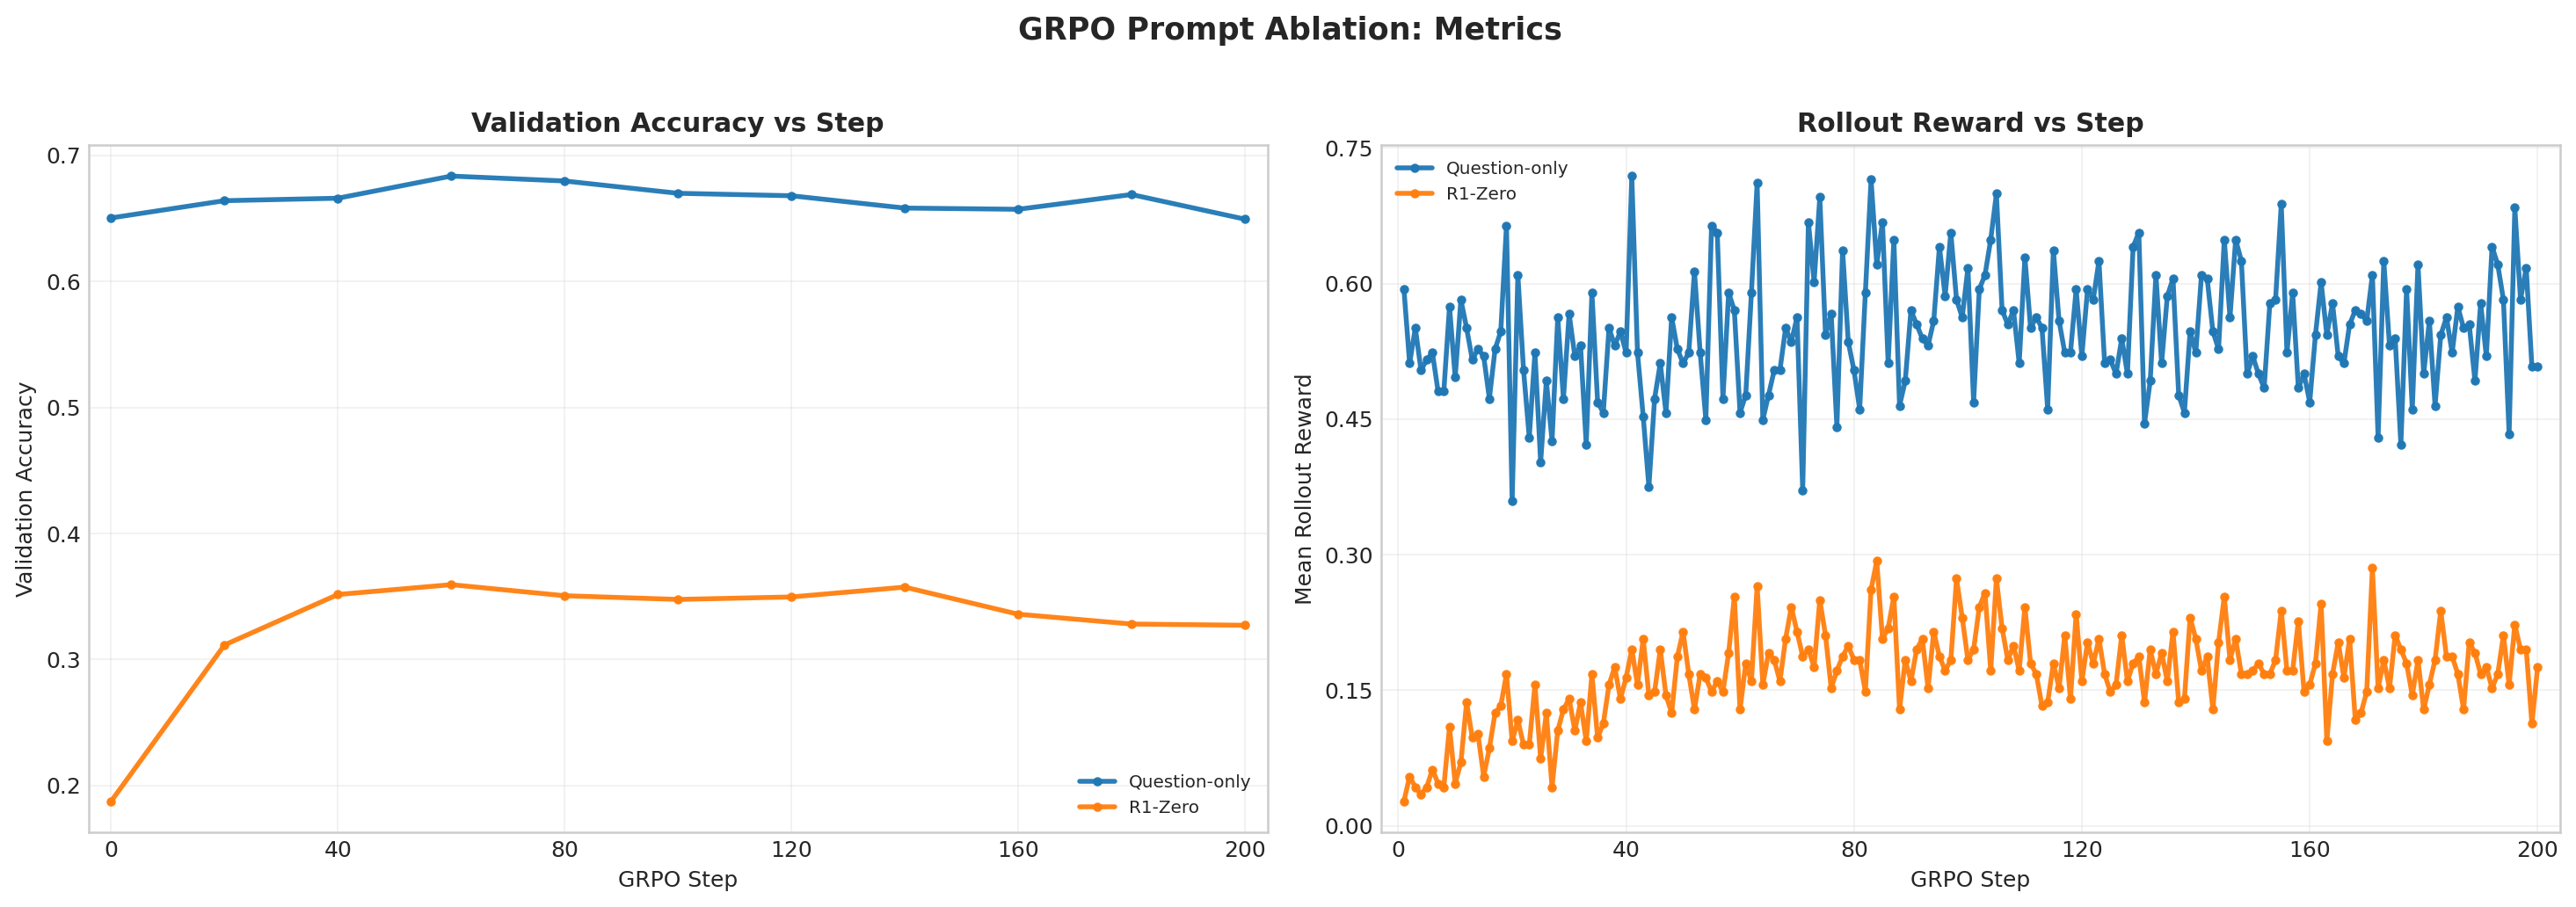
\includegraphics[width=0.8\textwidth]{section7_prompt_ablation.png}
			\caption{Prompt ablation: R1-Zero versus question-only.}
		\end{figure}
		
	\end{itemize}
	
	\appendix
	
	\section{Appendix}
	
	\subsection{Code Availability}
	
	All code mentioned in this report is available at \href{https://github.com/echung32/ece405-assignment3-alignment}{github.com/echung32/ece405-assignment3-alignment}.
	
	\subsection{VRAM Tuning Notes}
	
	For the GRPO runs, I used an AI agent to do short throughput and VRAM probes before launching longer experiments. Rather than guessing a larger training microbatch directly, the agent ran controlled 1-step and 2-step probes, inspected the resulting artifacts together with sampled \texttt{nvidia-smi} logs, and then recommended the next safe configuration to test. The full tuning note is available in the repository at \repofile{docs/VRAM_TUNING.md}{docs/VRAM\_TUNING.md}.
	
	The finding was that increasing training throughput by reducing \texttt{gradient\_accumulation\_steps} from 128 to 64 gave a large speedup while still preserving comfortable memory headroom on the GH200 training GPU. Pushing further to 32 was only slightly faster, but left too little margin for sustained runs and may lead to an unexpected OOM.
	
	\begin{table}[H]
		\centering
		\small
		\begin{tabular}{|l|c|c|c|c|l|}
			\hline
			Probe & Microbatch & Train update (s) & Step total (s) & Train GPU peak (GB) & Outcome \\
			\hline
			GA128 & 2 & 13.82 & 22.40 & 31.1 & Very safe, but under-utilized \\
			GA64 & 4 & 9.83 & 18.92 & 73.6 & Best safe operating point \\
			GA32 & 8 & 9.33 & 17.83 & 94.8 & Slightly faster, but too risky \\
			\hline
		\end{tabular}
		\caption{Short GH200 throughput probes used to tune GRPO VRAM usage.}
	\end{table}
	
	I also ran a 2-step confirmation probe at GA64, which remained stable on the second iteration and showed no additional phase-boundary memory blow-up. Based on those probes, the recommendation was \texttt{train\_batch\_size=256}, \texttt{gradient\_accumulation\_steps=64}.
	
	\subsection{Training Logs}
	
	Training curves and logged metrics are also available in Weights \& Biases at the following project pages:
	
	\begin{itemize}
		\item SFT: \url{https://wandb.ai/echung32-ece405/ece405-alignment-sft}
		\item Expert Iteration: \url{https://wandb.ai/echung32-ece405/ece405-alignment-expert-iteration}
		\item GRPO: \url{https://wandb.ai/echung32-ece405/ece405-alignment-grpo}
	\end{itemize}
	
\end{document}